
%% bare_conf.tex
%% V1.3
%% 2007/01/11
%% by Michael Shell
%% See:
%% http://www.michaelshell.org/
%% for current contact information.
%%
%% This is a skeleton file demonstrating the use of IEEEtran.cls
%% (requires IEEEtran.cls version 1.7 or later) with an IEEE conference paper.
%%
%% Support sites:
%% http://www.michaelshell.org/tex/ieeetran/
%% http://www.ctan.org/tex-archive/macros/latex/contrib/IEEEtran/
%% and
%% http://www.ieee.org/

%%*************************************************************************
%% Legal Notice:
%% This code is offered as-is without any warranty either expressed or
%% implied; without even the implied warranty of MERCHANTABILITY or
%% FITNESS FOR A PARTICULAR PURPOSE! 
%% User assumes all risk.
%% In no event shall IEEE or any contributor to this code be liable for
%% any damages or losses, including, but not limited to, incidental,
%% consequential, or any other damages, resulting from the use or misuse
%% of any information contained here.
%%
%% All comments are the opinions of their respective authors and are not
%% necessarily endorsed by the IEEE.
%%
%% This work is distributed under the LaTeX Project Public License (LPPL)
%% ( http://www.latex-project.org/ ) version 1.3, and may be freely used,
%% distributed and modified. A copy of the LPPL, version 1.3, is included
%% in the base LaTeX documentation of all distributions of LaTeX released
%% 2003/12/01 or later.
%% Retain all contribution notices and credits.
%% ** Modified files should be clearly indicated as such, including  **
%% ** renaming them and changing author support contact information. **
%%
%% File list of work: IEEEtran.cls, IEEEtran_HOWTO.pdf, bare_adv.tex,
%%                    bare_conf.tex, bare_jrnl.tex, bare_jrnl_compsoc.tex
%%*************************************************************************

% *** Authors should verify (and, if needed, correct) their LaTeX system  ***
% *** with the testflow diagnostic prior to trusting their LaTeX platform ***
% *** with production work. IEEE's font choices can trigger bugs that do  ***
% *** not appear when using other class files.                            ***
% The testflow support page is at:
% http://www.michaelshell.org/tex/testflow/



% Note that the a4paper option is mainly intended so that authors in
% countries using A4 can easily print to A4 and see how their papers will
% look in print - the typesetting of the document will not typically be
% affected with changes in paper size (but the bottom and side margins will).
% Use the testflow package mentioned above to verify correct handling of
% both paper sizes by the user's LaTeX system.
%
% Also note that the "draftcls" or "draftclsnofoot", not "draft", option
% should be used if it is desired that the figures are to be displayed in
% draft mode.
%
\documentclass[conference]{IEEEtran}
% Add the compsoc option for Computer Society conferences.
%
% If IEEEtran.cls has not been installed into the LaTeX system files,
% manually specify the path to it like:
% \documentclass[conference]{../sty/IEEEtran}




\usepackage{graphicx}
\usepackage{amssymb,url,times}%,subfigure}% amsthm is the one!
\usepackage{caption,subcaption,hyperref}
\usepackage{color,comment}
\usepackage{curves,pgfgantt}
\usepackage[linesnumbered,ruled,vlined]{algorithm2e} 




% Some very useful LaTeX packages include:
% (uncomment the ones you want to load)


% *** MISC UTILITY PACKAGES ***
%
%\usepackage{ifpdf}
% Heiko Oberdiek's ifpdf.sty is very useful if you need conditional
% compilation based on whether the output is pdf or dvi.
% usage:
% \ifpdf
%   % pdf code
% \else
%   % dvi code
% \fi
% The latest version of ifpdf.sty can be obtained from:
% http://www.ctan.org/tex-archive/macros/latex/contrib/oberdiek/
% Also, note that IEEEtran.cls V1.7 and later provides a builtin
% \ifCLASSINFOpdf conditional that works the same way.
% When switching from latex to pdflatex and vice-versa, the compiler may
% have to be run twice to clear warning/error messages.






% *** CITATION PACKAGES ***
%
%\usepackage{cite}
% cite.sty was written by Donald Arseneau
% V1.6 and later of IEEEtran pre-defines the format of the cite.sty package
% \cite{} output to follow that of IEEE. Loading the cite package will
% result in citation numbers being automatically sorted and properly
% "compressed/ranged". e.g., [1], [9], [2], [7], [5], [6] without using
% cite.sty will become [1], [2], [5]--[7], [9] using cite.sty. cite.sty's
% \cite will automatically add leading space, if needed. Use cite.sty's
% noadjust option (cite.sty V3.8 and later) if you want to turn this off.
% cite.sty is already installed on most LaTeX systems. Be sure and use
% version 4.0 (2003-05-27) and later if using hyperref.sty. cite.sty does
% not currently provide for hyperlinked citations.
% The latest version can be obtained at:
% http://www.ctan.org/tex-archive/macros/latex/contrib/cite/
% The documentation is contained in the cite.sty file itself.






% *** GRAPHICS RELATED PACKAGES ***
%
\ifCLASSINFOpdf
  % \usepackage[pdftex]{graphicx}
  % declare the path(s) where your graphic files are
  % \graphicspath{{../pdf/}{../jpeg/}}
  % and their extensions so you won't have to specify these with
  % every instance of \includegraphics
  % \DeclareGraphicsExtensions{.pdf,.jpeg,.png}
\else
  % or other class option (dvipsone, dvipdf, if not using dvips). graphicx
  % will default to the driver specified in the system graphics.cfg if no
  % driver is specified.
  % \usepackage[dvips]{graphicx}
  % declare the path(s) where your graphic files are
  % \graphicspath{{../eps/}}
  % and their extensions so you won't have to specify these with
  % every instance of \includegraphics
  % \DeclareGraphicsExtensions{.eps}
\fi
% graphicx was written by David Carlisle and Sebastian Rahtz. It is
% required if you want graphics, photos, etc. graphicx.sty is already
% installed on most LaTeX systems. The latest version and documentation can
% be obtained at: 
% http://www.ctan.org/tex-archive/macros/latex/required/graphics/
% Another good source of documentation is "Using Imported Graphics in
% LaTeX2e" by Keith Reckdahl which can be found as epslatex.ps or
% epslatex.pdf at: http://www.ctan.org/tex-archive/info/
%
% latex, and pdflatex in dvi mode, support graphics in encapsulated
% postscript (.eps) format. pdflatex in pdf mode supports graphics
% in .pdf, .jpeg, .png and .mps (metapost) formats. Users should ensure
% that all non-photo figures use a vector format (.eps, .pdf, .mps) and
% not a bitmapped formats (.jpeg, .png). IEEE frowns on bitmapped formats
% which can result in "jaggedy"/blurry rendering of lines and letters as
% well as large increases in file sizes.
%
% You can find documentation about the pdfTeX application at:
% http://www.tug.org/applications/pdftex





% *** MATH PACKAGES ***
%
\usepackage[cmex10]{amsmath}
% A popular package from the American Mathematical Society that provides
% many useful and powerful commands for dealing with mathematics. If using
% it, be sure to load this package with the cmex10 option to ensure that
% only type 1 fonts will utilized at all point sizes. Without this option,
% it is possible that some math symbols, particularly those within
% footnotes, will be rendered in bitmap form which will result in a
% document that can not be IEEE Xplore compliant!
%
% Also, note that the amsmath package sets \interdisplaylinepenalty to 10000
% thus preventing page breaks from occurring within multiline equations. Use:
%\interdisplaylinepenalty=2500
% after loading amsmath to restore such page breaks as IEEEtran.cls normally
% does. amsmath.sty is already installed on most LaTeX systems. The latest
% version and documentation can be obtained at:
% http://www.ctan.org/tex-archive/macros/latex/required/amslatex/math/


\newtheorem{prop}{Proposition}
\newcommand{\norm}[1]{\ensuremath{\left\| #1 \right\|}}
\newcommand{\abs}[1]{\ensuremath{\left| #1 \right|}}
\newcommand{\bracket}[1]{\ensuremath{\left[ #1 \right]}}
\newcommand{\braces}[1]{\ensuremath{\left\{ #1 \right\}}}
\newcommand{\parenth}[1]{\ensuremath{\left( #1 \right)}}
\newcommand{\ip}[1]{\ensuremath{\langle #1 \rangle}}
\newcommand{\refeqn}[1]{(\ref{eqn:#1})}
\newcommand{\reffig}[1]{Figure \ref{fig:#1}}
\newcommand{\tr}[1]{\mbox{tr}\ensuremath{\negthickspace\bracket{#1}}}
\newcommand{\trs}[1]{\mbox{tr}\ensuremath{\!\bracket{#1}}}
\newcommand{\deriv}[2]{\ensuremath{\frac{\partial #1}{\partial #2}}}
\newcommand{\G}{\ensuremath{\mathsf{G}}}
\newcommand{\SO}{\ensuremath{\mathsf{SO(3)}}}
\newcommand{\T}{\ensuremath{\mathsf{T}}}
\renewcommand{\L}{\ensuremath{\mathsf{L}}}
\newcommand{\so}{\ensuremath{\mathfrak{so}(3)}}
\newcommand{\SE}{\ensuremath{\mathsf{SE(3)}}}
\newcommand{\se}{\ensuremath{\mathfrak{se}(3)}}
\renewcommand{\Re}{\ensuremath{\mathbb{R}}}
\newcommand{\Sph}{\ensuremath{\mathsf{S}}}
\newcommand{\aSE}[2]{\ensuremath{\begin{bmatrix}#1&#2\\0&1\end{bmatrix}}}
\newcommand{\ase}[2]{\ensuremath{\begin{bmatrix}#1&#2\\0&0\end{bmatrix}}}
\newcommand{\D}{\ensuremath{\mathbf{D}}}
\renewcommand{\d}{\ensuremath{\mathbf{d}}}
\newcommand{\pair}[1]{\ensuremath{\left\langle #1 \right\rangle}}
\newcommand{\met}[1]{\ensuremath{\langle\!\langle #1 \rangle\!\rangle}}
\newcommand{\Ad}{\ensuremath{\mathrm{Ad}}}
\newcommand{\ad}{\ensuremath{\mathrm{ad}}}
\newcommand{\g}{\ensuremath{\mathfrak{g}}}
\newcommand{\argmin}{\operatornamewithlimits{argmin}}
\newcommand{\argmax}{\operatornamewithlimits{argmax}}
\newcommand{\WriteBlue}[1]{{\color{blue}\protect #1}}
\graphicspath{{./Fig/}}



% correct bad hyphenation here
\hyphenation{op-tical net-works semi-conduc-tor}


\begin{document}
%
% paper title
% can use linebreaks \\ within to get better formatting as desired
\title{Autonomous Quadrotor 3D Mapping and Exploration Using Exact Occupancy Probabilities}

% for over three affiliations, or if they all won't fit within the width
% of the page, use this alternative format:
% 
\author{\IEEEauthorblockN{Evan Kaufman\IEEEauthorrefmark{1},
Kuya Takami\IEEEauthorrefmark{1},
Zhuming Ai\IEEEauthorrefmark{2} and
Taeyoung Lee\IEEEauthorrefmark{1}}
\IEEEauthorblockA{\IEEEauthorrefmark{1}Department of Mechanical and Aerospace Engineering\\
The George Washington University, Washington, DC 20052\\
Email: \{evankaufman, kuya, tylee\}@gwu.edu}
\IEEEauthorblockA{\IEEEauthorrefmark{2}Information Management \& Decision Architectures
\\ U.S. Naval Research Laboratory, Washington, DC 20375}
}

\maketitle


\begin{abstract}
%Robotic mapping and exploration have received significant attention recently because exploring uncertain environments can pose danger to humans, and robots can produce highly detailed maps. Commonly uncertain environments contain complex geometries and robots frequently face restrictive terrains, motivating a 3D representation of mapping from a vehicle capable of hover. 

This paper deals with the aerial exploration for an unknown three-dimensional environment, where Bayesian probabilistic mapping is integrated with a stochastic motion planning scheme to minimize the map uncertainties in an optimal fashion. We utilize the popular occupancy grid mapping representation, with the goal of determining occupancy probabilities of evenly-spaced grid cells in 3D with sensor fusion from multiple depth sensors with realistic sensor capabilities. The 3D exploration problem is decomposed into 3D mapping and 2D motion planning for efficient real-time implementation. This is achieved by projecting important aspects of the 3D map onto 2D maps, where a predicted level of map uncertainty, known as Shannon's entropy, provides an exploration policy that governs robotic motion. Both mapping and exploration algorithms are demonstrated with both numerical simulations and quadrotor flight experiments.
\end{abstract}

\section{Introduction}

Robotic mapping is the process of generating maps representing the environment surrounding a robot.
Mapping serves an important role in tasks such as search-and-rescue, surveillance, and robotic cleaning.
Several grid-based map representations have been studied, e.g.,~\cite{WolSuk05,MeyBeiBur12,TanThoWolBus14}, because they provide abundant occupancy knowledge about the environment and are computationally tractable. 

Most grid-based mapping representations are designed for 2D, while others are extended to capture a full 3D environment. In particular, occupancy probabilities have been assigned to a uniform 3D grid in~\cite{Andert09,PirRutBisSch11}. Another highly-popular variation of occupancy grid mapping is the Octomap representation~\cite{WurHorBenStaBur10,HorWurBenStaBur13}, which has added features such as extending the mapping limits and changing cell sizes. 

However, these approaches are based on an approximate solution of the inverse sensor model, to determine the occupancy probabilities based on the depth sensor measurements. As such, the prior belief of the environment and the stochastic properties of the sensor are not properly accounted. Another popular approach for the inverse sensor model involves a simulated learning technique~\cite{Thr01,ThrBurFox05,SouMaiGon12}, but this is not suitable for the higher dimensional configurations composed of maps, poses, and measurement due to the large number of required samples. None of these approaches use the sensor properties to directly obtain a Bayesian solution to occupancy probability.

%        1.      sensor fusion in mapping
The approximate nature of the occupancy probability motivates an exact Bayesian solution that can be applied in 3D. This paper proposes a computationally-efficient algorithm to obtain the exact solution to the inverse sensor problem to generate probabilities in a 3D environment, following the framework of~\cite{KauLeeAiMos16,KauTakAiLee17}. The proposed approach integrates all of the stochastic information available for the environment, such as the prior map estimate and multiple sensor measurements, according to the Bayesian framework, to obtain the exact 3D occupancy probabilities. As such, it provides a unified framework for sensor fusion between multiple sensors with various properties, such as sensor accuracy, and fields of view. 

%        2.      proposing a method to combine 3D mapping and 2D exploration: Also, we need to motivate why we are not doing full 3D exploration. Stress that we are proposing a computationally friendly approach to perform 3D mapping with projection using the fact there is less variation in the floor plan along the vertical direction.
The second topic of this paper deals with autonomous exploration, which provides the policies that govern robotic motion. A common approach is known as frontier-based exploration, proposed for 2D environments in~\cite{Yam97,Yam98} and extended to 3D  using the Octomap representation in~\cite{ZhuDinLinWu15,SenWan16,KleDor13}, and similarly using a visibility metric in~\cite{SawKriSri09}. This approach moves robots toward the boarder between certain and uncertain spaces, though these systematic actions are not based on any consideration of the future probabilistic map uncertainty.

Alternatively, there have been exploration techniques that are based on a quantitative measure of uncertainty known as Shannon's entropy~\cite{StaGriBur05}, and it is used to acquire expected map information gain in~\cite{KauAiLee16,KauTakAiLee17}. This paper focusses on extending these concepts to 3D in a numerically efficient manner.  The prescribed 3D exact inverse sensor model is critical in computing the expected information gain precisely. There are several challenges with obtaining expected information gain of 3D measurement scans, particularly due to the extended computational load. Considering the typically low variation in floor plans along the vertical direction, this paper proposes a numerically efficient scheme that projects stochastic properties of the 3D probabilistic occupancy grid to 2D spaces for optimal information gain and collision avoidance. This exploits the important characteristics of 3D maps. This process of combining 3D mapping and 2D exploration is completed in a computationally-efficient manner.

%        3.      hardware/software for aerial exploration experiment.
Finally, we present both numerical simulations and flight experiments for the proposed exploration schemes. The multiple tasks of sensor data acquisition, mapping, exploration, flight control, and communications are implemented with Python/C++, to be executed simultaneously in a ROS environment. They are verified with a quadrotor unmanned aerial vehicle operated by the NVidia Jetson computing module with an ASUS Xtion infrared depth sensor and Hokuyo laser scanner. 

The paper is organized as follows. The problem is formulated in Section II. Special considerations for mapping and exploration in 3D are established in Section III. A numerical example is demonstrated in Section IV. Experimental results are shown in Section V, followed by conclusions and future work.



%% Prior to TLee edits:
%Robotic mapping is the process of generating maps representing the environment surrounding a robot.
%Mapping serves an important role in tasks such as search-and-rescue, surveillance, and robotic cleaning.
%Several grid-based map representations have been studied, e.g.,~\cite{WolSuk05,MeyBeiBur12,TanThoWolBus14}, because they provide abundant occupancy knowledge about the environment and are computationally tractable. 
%
%Most grid-based mapping representations are designed for 2D, while others are extended to capture a full 3D environment. In particular, occupancy probabilities have been assigned to a uniform 3D grid in~\cite{Andert09,PirRutBisSch11}. Another highly-popular variation of occupancy grid mapping is the Octomap representation~\cite{WurHorBenStaBur10,HorWurBenStaBur13}, which has added features such as extending the mapping limits and changing cell sizes. However, Octomaps, and the 3D uniform grid-based approaches mentioned above, produce cell occupancy probabilities that do not directly depend on the depth sensor stochastic properties. Instead, these approaches determine occupancy probabilities using an approximate function. Another method introduced in~\cite{Thr01,ThrBurFox05} and implemented in 3D with~\cite{SouMaiGon12} uses a simulated learning technique to find these probabilities, which may be difficult over the large dimensional space composed of maps, poses, and measurements. An additional approach such as~\cite{TanThoWolBus14} applies a particle filter to estimate the map. None of these approaches use the sensor properties to directly obtain a Bayesian solution to occupancy probability.
%
%%        1.      sensor fusion in mapping
%The approximate nature of the occupancy probability motivates an exact Bayesian solution that can be applied in 3D. This paper proposes a computationally-efficient algorithm that follows the framework of~\cite{KauLeeAiMos16,KauTakAiLee17} to generate probabilities in a 3D environment. Since this approach only requires the origin and direction of sensor measurements to be known, the algorithm is designed to work for any number of sensors. Sensor fusion from several sources can provide important information about the environment with different levels of sensor certainty, fields of view, and vantage points.
%
%%        2.      proposing a method to combine 3D mapping and 2D exploration: Also, we need to motivate why we are not doing full 3D exploration. Stress that we are proposing a computationally friendly approach to perform 3D mapping with projection using the fact there is less variation in the floor plan along the vertical direction.
%The second topic of this paper deals with autonomous exploration, which provide the policies that govern robotic motion. A common approach is known as frontier-based exploration, proposed for 2D environments in~\cite{Yam97,Yam98} and extended to 3D with~\cite{ZhuDinLinWu15,SenWan16,KleDor13} using the Octomap representation, and similarly in~\cite{SawKriSri09} using a visibility metric. This approach moves robots toward the boarder between certain and uncertain space, though these systematic actions are not based on any consideration of the future probabilistic map uncertainty. Alternatively, there have been exploration techniques that are based on a quantitative measure of uncertainty known as Shannon's entropy~\cite{StaGriBur05}, an uncertainty metric based on grid cell occupancy probabilities. Shannon's entropy is used to acquire expected map information gain in~\cite{KauAiLee16,KauTakAiLee17}, and this paper focusses on extending these concepts to 3D. There are several challenges with obtaining expected information gain of 3D measurement scans, particularly as they relate to computational load. Considering the typically low variation in floor plans that robots explore during indoor explorations, this paper proposes two methods to generate 2D exploration maps that exploit the important characteristics of 3D maps. This process of combining 3D mapping and 2D exploration is completed in a computationally-efficient manner.
%
%%        3.      hardware/software for aerial exploration experiment.
%Finally, this paper comments on the hardware and software necessary to implement these challenging algorithms for an aerial mapping and exploration experiment. This paper provides the basic software structure and features for mapping and generating exploration trajectories on a host computer while running depth sensors and a flight controller onboard a mobile robot.
%
%The paper is organized as follows. The problem is formulated in Section II. Special considerations for mapping and exploration in 3D are established in Section III. A numerical example is demonstrated in Section IV. Experimental results are shown in Section V, followed by conclusions and future work.


\section{Problem Formulation}

The key differences between the approaches presented in this paper and others relate to how map cell occupancy probabilities and measurement ray entropies are calculated directly from a priori cell probabilities and stochastic properties of the sensors involved. These are defined next.

\subsection{Probabilistic Occupancy Grid Mapping}
\label{subsec:POGM}
Let a map $m$ be an occupancy grid map decomposed into $n$ evenly-spaced cubic grid cells with fixed edge length $\alpha$. The $i$-th grid cell is assigned to a static binary random variable $\mathbf{m}_i$ for $i\in\braces{1,2,\ldots,n}$, that is defined as $\mathbf{m}_i=1$ when occupied, and $\mathbf{m}_i=0$ when free. The location and size of each grid cell is assumed known, where a smaller cell size better represents a space, but increases computation and memory. Therefore, a map $m$ is defined by $\{\mathbf{m}_1,\ldots, \mathbf{m}_{n}\}$ ($2^{n}$ possible maps).

Another random variable is defined as $\bar{\mathbf{m}}_i=1-\mathbf{m}_i$ for convenience, which is the event that the $i$-th cell is free, i.e., $P(\bar{\mathbf{m}}_i)=1-P(\mathbf{m}_i)$. The random variables composing $m$ are assumed mutually independent, 
\begin{align}
P(m)=P(\mathbf{m}_1,\mathbf{m}_2,\ldots,\mathbf{m}_{n})=\prod_{i=1}^{n}P(\mathbf{m}_i).
\end{align}

% {R ? R3�3 | RT R = I, det R = 1}
Consider a range sensor that provides scans of the surrounding environment in order to identify the closest occupied space. Let the measurement scan at the $t$-th time step be $Z_t$, where $z\in Z_t$ is a single measurement ray. Let the $t$-th pose be denoted by $X_t=\braces{x_t,R_t}$ with location $x_t\in\Re^3$ and attitude $R_t\in\SO=\braces{R\in\Re^{3\times3}|R^\T R=I,\det{R}=1}$, where $X_t$ is assumed to be known. Given the sensor probabilistic properties $p(z|X_t,m)$, commonly referred to as the \emph{forward sensor model}, the goal is finding the \emph{inverse sensor model}, $P(m|z,X_{1:t},Z_{1:t-1})$. To obtain this probability for all cells,~\cite{KauLeeAiMos16,KauTakAiLee17} introduced a reduced map $r\subset m$ composed of $n_r$ cells along $z$, where cells are indexed by increasing distance from $x_t$, and $\mathbf{r}_{k+}$ refers to the event that the $k$-th cell of map $r$ is the closest occupied space. Then, the inverse sensor model for the $k$-th cell is
\begin{align}
\label{eqn:RayISMAnswer}
P(\mathbf{r}_{k}|z,X_{1:t},Z_{1:t-1})&=\eta\tilde P(\mathbf{r}_{k}|z,X_{1:t},Z_{1:t-1}),
\end{align}
where the unnormalized probability of the inverse sensor model is defined as
\begin{align}
\label{eqn:Unnormalized}
\tilde P(\mathbf{r}_{k}|z,X_{1:t},&Z_{1:t-1})\nonumber\\
&=\mathbf{P}_k^-
\bigg[\sum_{i=1}^{k-1}\bigg\{\prod_{j=0}^{i-1}\bar{\mathbf{P}}_j^-\bigg\}p(z|\mathbf{r}_{i+},X_t)\mathbf{P}_k^-\bigg]\nonumber\\
&\quad + \bigg\{\prod_{j=0}^{k-1}\bar{\mathbf{P}}_j^-\bigg\}p(z|\mathbf{r}_{k+},X_t)\mathbf{P}_k^-,
\end{align}
where a priori probability is $\mathbf{P}_k^-=P(\mathbf{r}_{k}|X_{1:t-1},Z_{1:t-1})$, its complement is $\bar{\mathbf{P}}_k^-=1-\mathbf{P}_k^-$, $P(\bar{\mathbf{r}}_{0}|X_{1:t-1},Z_{1:t-1})=P(\mathbf{r}_{n_r+1}|X_{1:t-1},Z_{1:t-1})=1$ for convenience, and $p(z|\mathbf{r}_{(n_r+1)+},X_t)$ represents the forward sensor model of a maximum sensor reading. The normalizer $\eta$ is given by
\begin{align}
\label{eqn:allEta}
\eta
&=
\bigg[\sum_{i=1}^{n_{r}+1}\bigg\{\prod_{j=0}^{i-1}\bar{\mathbf{P}}_j^-\bigg\} p(z|\mathbf{r}_{i+},X_t)\mathbf{P}_k^-\bigg]^{-1},
\end{align}
and it is independent of the cell index $k$. Since the terms of \refeqn{Unnormalized} are easily obtained and several are used repeatedly to obtain \refeqn{allEta}, the computational cost of \refeqn{RayISMAnswer} is trivial and can be applied in real-time. This process is repeated for all measurements composing scan $Z_t$.

\subsection{Predictive Entropy-Based Autonomous Exploration}


Since occupancy grid mapping provides a probabilistic representation of surrounding space, this mapping scheme holds probabilistic information about the uncertainty of the map. Shannon's entropy is commonly used as a measure of uncertainty, such as in~\cite{StaGriBur05}. Given the probabilities of each grid cell of map $m$, Shannon's entropy of an individual cell and the entire map are defined as
\begin{align}
\label{eqn:ShannonsEntropyCell}
H(P(\mathbf{m}_i))&=-P(\mathbf{m}_i)\log{P(\mathbf{m}_i})-P(\bar{\mathbf{m}}_i)\log{P(\bar{\mathbf{m}}_i}),
\\
\label{eqn:ShannonsEntropyMap}
H(P(m))&=\sum_{i=1}^{n_m}H(P(\mathbf{m}_i)),
\end{align}
respectively.
The entropy of the $i$-th grid cell is maximized when $P(\mathbf{m}_i)=0.5$ (greatest uncertainty) and minimized as $P(\mathbf{m}_i)$ approaches $0$ or $1$ (smallest uncertainty). %; thus Shannon's entropy is a measure of uncertainty.

Let an unvisited candidate future pose and its measurement scan be $X_c$ and $Z_c$, respectively. Since the robot has not visited $X_c$, any change to the probabilistic map must be predicted. Much like the probabilistic mapping, this is achieved ray-by-ray~\cite{KauAiLee16,KauTakAiLee17}. Since all grid cell probabilities are conditioned on the history of poses $X_{1:t}$ and measurement scans $Z_{1:t}$, these are removed from the remaining equations for simplicity. For candidate ray $z_c$, the expected entropy is
\begin{align}
\label{eqn:DiscExpEntropyRay}
&\text{E}[H(P(m|x_c,z_{c}))]=\sum_{k=1}^{n_{r}+1}\bigg\{H(P(m|x_c,z_{c,k}))P(z_{c,k}|x_c)\bigg\},
\end{align}
where subscript $k$ refers to the event that the candidate \emph{measurement} captures the $k$-th cell along the ray, i.e., $z_{c,k}$ is the distance from $x_c$ to the $k$-th grid cell. The first term of the summation of \refeqn{DiscExpEntropyRay}, namely $H(P(m|x_c,z_{c,k}))$, is obtained with the inverse sensor model \refeqn{RayISMAnswer}--\refeqn{allEta} and entropy definitions \refeqn{ShannonsEntropyCell}, \refeqn{ShannonsEntropyMap}. The second term is found using \refeqn{allEta} with
\begin{align}
P(z_{c,k}|x_c)&=\frac{p(z_{c,k}|x_c)}{\sum_{i=1}^{n_{r}+1}p(z_{c,i}|x_c)}=\frac{\eta_{c,k}^{-1}}{\sum_{i=1}^{n_{r}+1}\eta_{c,i}^{-1}},
\end{align}
where $\eta_{c,k}$ refers to the normalizer calculated with $z_{c,k}$.
The goal of entropy-based autonomous exploration is to select the optimal pose $X^*_c$ that maximizes the expected information gain,
\begin{align}
\label{eqn:objectiveFunOptimized}
X_c^*&=\argmax_{X_c}{\ \mathcal I(X_c)},
\\
\label{eqn:objectiveFun}
\mathcal I(X_c)&=H(P(m|X_{1:t},Z_{1:t}))-\text{E}\left[H(P(m|X_c,Z_c))\right],
\end{align}
where \refeqn{DiscExpEntropyRay} is used repeatedly for several sample rays that compose scan $Z_c$ as shown in~\cite{KauAiLee16}.

Once an optimal pose $X^*_c$ is selected, a set of collision-free waypoints along the occupancy grid is easily obtained with Dijkstra's algorithm~\cite{Dij59}. Then, a constrained least squares optimization provides a trajectory as a tracking command for the robot controller.

\section{Mapping and Exploring in 3D}

\subsection{Mapping in 3D Space}

The inverse sensor model from~\cite{KauLeeAiMos16,KauTakAiLee17} is based on an arbitrary vector spanning 2D space. The distances from the robot to grid cells are obtained geometrically through ray casting. This method is easily extended to 3D space, and the inverse sensor model is applied identically. Since the map is updated ray-by-ray (each measurement ray is considered once by itself), this approach is extended for measurement fusion of any number of sensors; the map is updated by each ray of a scan sequentially, then the map is updated by the rays of the next scan in queue, which might have different characteristics. There are several reasons why a robot might be equipped with multiple sensors, e.g., different fields-of-view or depth sensor properties. The proposed 3D mapping approach can handle measurements from different sources with different properties.

However, implementation in 3D requires several careful considerations. First, the number of cell occupancy probabilities tracked with computer memory increases by a factor of the number of cells in the added dimension. In its current form, the proposed method assumes fixed map limits, so these should be carefully selected with grid cell resolution based on available memory. Second, measurement rays spanning 3D space typically involve more intersections with grid cells. The computational order of ray casting and the inverse sensor model are proportional to the number of grid cells along the ray $n_r$, so careful consideration must be placed on sensor limits and rays per scan that can be considered. Typically, computers small enough to be carried onboard flying robots lack the memory or processing capabilities to update massive maps quickly. Therefore, an onboard computer can simply stream the sensor data, and a more powerful computer can run the mapping.

Additionally, aerial vehicles are frequently subject to fast movements, and the time stamps for pose estimates and depth sensor readings are not guaranteed to align. For example, the most recent pose estimate and measurement scan may have significantly different time stamps while the robot is rapidly rotating. Using these together violates the assumption that the robot pose is well-known for every measurement scan, i.e., $X_t$ and $Z_t$ are given. Therefore, pose estimates and sensor readings must be paired according to their time stamps. A useful tool that easily satisfies this goal is message filtering with the Robot Operating System (ROS), where stamped poses and measurement scans are synchronized using recently received data.

\subsection{Autonomous Exploration in 3D Space}

The goal of the proposed autonomous exploration strategy is moving to poses that maximize the information the robot expects to learn about the map, measured with entropy. To achieve this in real-time, careful consideration is placed on computational costs. In particular, the expected entropy computational order of a ray that intersects $n_r$ cells is $(n_r+1)^2$. Since most quadrotor flight is close to hover and floor plans exhibit little variation in the vertical direction, the proposed exploration uses 2D occupancy grid maps located at the desired exploration height. This approach decreases $n_r$ and simplifies the exploration problem with 3D space. These 2D maps project important properties of the 3D map.

\subsubsection{Collision and Entropy Maps}
Occupancy grid map cell volume is frequently smaller than the size of the robot taking measurements, particularly with highly-detailed maps. This motivates a method to simply represent locations that risk collision, referred to as a \emph{collision map} $C$. Let $k_C\geq1$ be an integer representing the minimum number of 3D grid cells that form a cube that can completely encompass the robot, i.e., the collision map cell edge length is
\begin{align}
\label{eqn:alphaC}
\alpha_C=k_C\alpha.
\end{align}
Consider the set $m_{C,k}\subset m$ consisting of the 3D grid cells falling inside the limits of the $k$-th cell of collision map $C$, namely $\mathbf{C}_k$. Then the collision probability is
\begin{align}
P(\mathbf{C}_k)=\max{(P(\mathbf{m}_i)\ \forall \ i\in m_{C,k})}.
\end{align}
Then, the robot is only allowed to consider moving into $k$-th cell of the collision map if
\begin{align}
P(\mathbf{C}_k) \leq C_\text{thresh},
\end{align}
where $C_\text{thresh}>0$ is a maximum acceptable collision threshold, typically chosen slightly greater than $0$. In short, this conservative approach limits robotic motion to regions with a low risk of collision while neglecting objects far above or below the exploration plane.

In a similar method, \emph{entropy map} $E$ determines cells based on the entropy metric of \refeqn{ShannonsEntropyCell} over a different subset of cells. Let the $E$ be a 2D map composed of cells with edge length $\alpha$ located at the exploration height. Let the set $m_{E,k}\subset m$ be the cells directly above and below the $k$-th cell of $E$, neglecting any 3D cells located lower than the floor height. Selecting this set is advantageous because measurements are assumed not to penetrate occupied cells (edge length $\alpha$) and measurement rays are typically not closely-aligned with the third axis of the inertial frame (vertically long set). Furthermore, any cells located below the floor, which cannot be reached, should not impact the uncertainty of the space. Then, the occupancy probability of the $k$-th entropy map cell is selected as
\begin{align}
\label{eqn:ProbEntropyMap}
P(\mathbf{E}_k)=\argmax_{P(\mathbf{m}_i)}(H(P(\mathbf{m}_i))\ \forall \ i\in m_{E,k}).
\end{align}
After several measurements of the cells belonging to $m_{E,k}$, it is common for $H(P(\mathbf{E}_k))\approx0$, which implies that these cells are well-known. However, this does not imply that the captured space is \emph{entirely} free or occupied (e.g. an object on the ground that does not breach the upper map boundary), so applying \refeqn{ProbEntropyMap} alone could arbitrarily set $P(\mathbf{E}_k)$ close to $0$ or $1$. This can have damaging effects on the expected information of cells beyond the $k$-th cell. Let $P_\text{min}>0$ be a lower bound such that $H(P_\text{min})=H(1-P_\text{min})\approx0$. If $H(P(\mathbf{E}_k))\leq H(P_\text{min})$, then this probability is corrected to
\begin{align}
P(\mathbf{E}_k)= 
\begin{cases}
    P_\text{min},			& \text{if } \text{mean}(P(\mathbf{m}_i)\ \forall \ i\in m_{E,k})\leq0.5\\
    1-P_\text{min},              & \text{otherwise}
\end{cases},
\end{align}
where the first case corresponds to mostly open space and the second case corresponds to mostly occupied space (e.g. walls and objects). In short, the candidates are only considered if they can be reached over collision map $C$ via Dijkstra's search, and the information gains of the reachable candidates are predicted using entropy map $E$.

\subsubsection{Collision and Entropy Combination Map}
The second proposed technique combines the advantages of both the collision and entropy maps into a 2D projected occupancy grid map, which can be used for both tasks. Let the \emph{collision and entropy combination map} $B$ be a 2D projected map located at the exploration height with grid cell edges the same as the collision map, namely $\alpha_C$ from \refeqn{alphaC}, using the same subset of grid cells from the collision map, namely $m_C$. Considering that the cells begin with uniform probability $P_\text{init}$ where $0<P_\text{init}<1$, define a threshold $P_\text{thresh}$ such that $P_\text{init}<P_\text{thresh}<1$. Then, the probability assigned to the $k$-th grid cell of $B$ is
\begin{align}
P(\mathbf{B}_k)= 
\begin{cases}
    P(\mathbf{C}_k),			& \text{if }P(\mathbf{C}_k)\geq P_\text{thresh}\\
    \min{(P(\mathbf{m}_i)\ \forall \ i\in m_{C,k})},              & \text{otherwise}
\end{cases}.
\end{align}

This approach has several advantages. First, measurements must enter the vicinity of the $k$-th cell for $P(\mathbf{B}_k)$ to change from $P_\text{init}$. Without prior measurements, capturing $P(\mathbf{B}_k)$ produces a large reward for the expected information gain in \refeqn{objectiveFun}. Second, the value of $P_\text{thresh}$ can be modified based on how conservative the collision risk assessment for a robot should be. Additionally, when $P(\mathbf{B}_k)<P_\text{thresh}$, this event tends to favor free cells such that expected information gains of cells beyond the $k$-th cell have greater impact on exploration. Furthermore, a single map is simpler, and since cell sizes satisfy $\alpha_C\geq\alpha$, it follows that $n_r$ can only be decreased with $\alpha_C$, thereby increasing computational speed.

\section{Numerical Results}

\subsection{Software Structure}
%        A.      Software Structures
%                list and explain ROS nodes

The Robot Operating System (ROS) provides an excellent framework for several programs, referred to as \emph{nodes}, to communicate easily. These are mostly coded in C++ for speed, except for a few Python scripts for a GUI and trivial message conversions, and launch/yaml scripts for running nodes and setting parameters. 

Gazebo serves as the simulator node, with plugins to simulate an Asus Xtion color depth sensor and a Hokuyo LIDAR. Gazebo also provides position and attitude transforms from the world to the quadrotor body, and the ability to set robot model states directly. 

Using fixed transforms between the quadrotor body and its onboard sensors, an original mapping node uses a variation of ROS message filters, known as transform message filters, to synchronize the sensor poses with sensor readings. These serve as inputs for ray casting in 3D, which provides the cell probabilities and depths along the ray through geometry. Then, the inverse sensor model serves to update the map ray-by-ray.  The node is designed to work for any number of sensors, specified by sensor parameters in a yaml configuration file.

There are two processes for exploration. The first process is projecting the 3D map onto 2D maps; the same code under different conditional parameters produces two nodes, for collision and entropy maps. The second process subscribes to these two 2D maps; the collision map serves as input for candidate pose consideration and Dijstra's search, and the entropy map is used to predict expected information gain. This node provides path messages, composed of desired poses $0.01$sec apart, that are easily visualized with the ROS visualization package, Rviz.

Finally, a path-interpreter node subscribes to the path messages and interpolates the pose at the current ROS time step. This pose is converted into a message that sets the Gazebo quadrotor state.


\subsection{Simulation Results}
%        B.      Simulation Results
%                a little bit more interpretations for the results

The 3D mapping and exploration algorithms are simulated with several parameters.  In particular, the Xtion and Hokuyo are modeled using normalized Gaussian and uniform distributions for the sensor model, with a Gaussian probability of $0.9$ with $\sigma_\text{Xtion}=0.25$m and $\sigma_\text{Hokuyo}=0.1$m, respectively, which are greater than their specified values to account for pose uncertainty and distortion with the Xtion. Since the Xtion tends to distort depths significantly beyond $4$m, this maximum reading considered for both the Xtion and Hokuyo, and the uniform distribution (probability $0.1$) covers the sensor ranges from $0.5$m to $4$m. A cell size of $\alpha=0.075$m is selected and the map limits are $-4$m to $4$m in the x-direction, $-6$m to $6$m in the y-direction, and $-0.15$m to $1.5$m in the z-direction. The initial probability of cells is selected at $P_\text{init}=0.1$. For the collision map, the cell edge factor is $k_C=3$. Additionally, Dijkstra's algorithm produces a cost map composed of distance costs for each collision map cell, denoted $d_\text{cell}$, from the current robot position to the candidate pose locations over a collision-free path about the occupancy grid. A normalized variation on the \emph{bump function}~\cite{Joh06} with maximum distance $d_\text{max}>0$,% TODO: CHECK!
\begin{align}
\label{eqn:bumpFun}
\text{bump}(d_\text{cell})= 
\begin{cases}
    e^{1-\frac1{1-(d_\text{cell}/d_\text{max})^2}},			& \text{if }-d_\text{max}<d_\text{cell}<d_\text{max}\\
    0,              				& \text{otherwise}
\end{cases},
\end{align}
is multiplied to \refeqn{objectiveFun} when optimizing \refeqn{objectiveFunOptimized}. For this experiment, $d_\text{max}$ is chosen as the maximum value of $d_\text{cell}$ on the cost map. This serves to prioritize understanding the local surrounding space before the robot moves across the map to distant regions, while still considering all of the pose candidates.

In the simulation, the robot explores the simulated environment for $8$min while taking measurements. The 3D occupancy grid map and true environment are shown in Fig. \ref{fig:sim3DMap}. The Gazebo simulated environment and two 2D projected maps for collision and entropy are shown in Fig. \ref{fig:sim2Dmaps}. The total map entropy as a function of time is shown in Fig. \ref{fig:simH}.


\begin{figure}[!t]
    	\begin{subfigure}[t]{0.24\columnwidth}
           	\centering
          	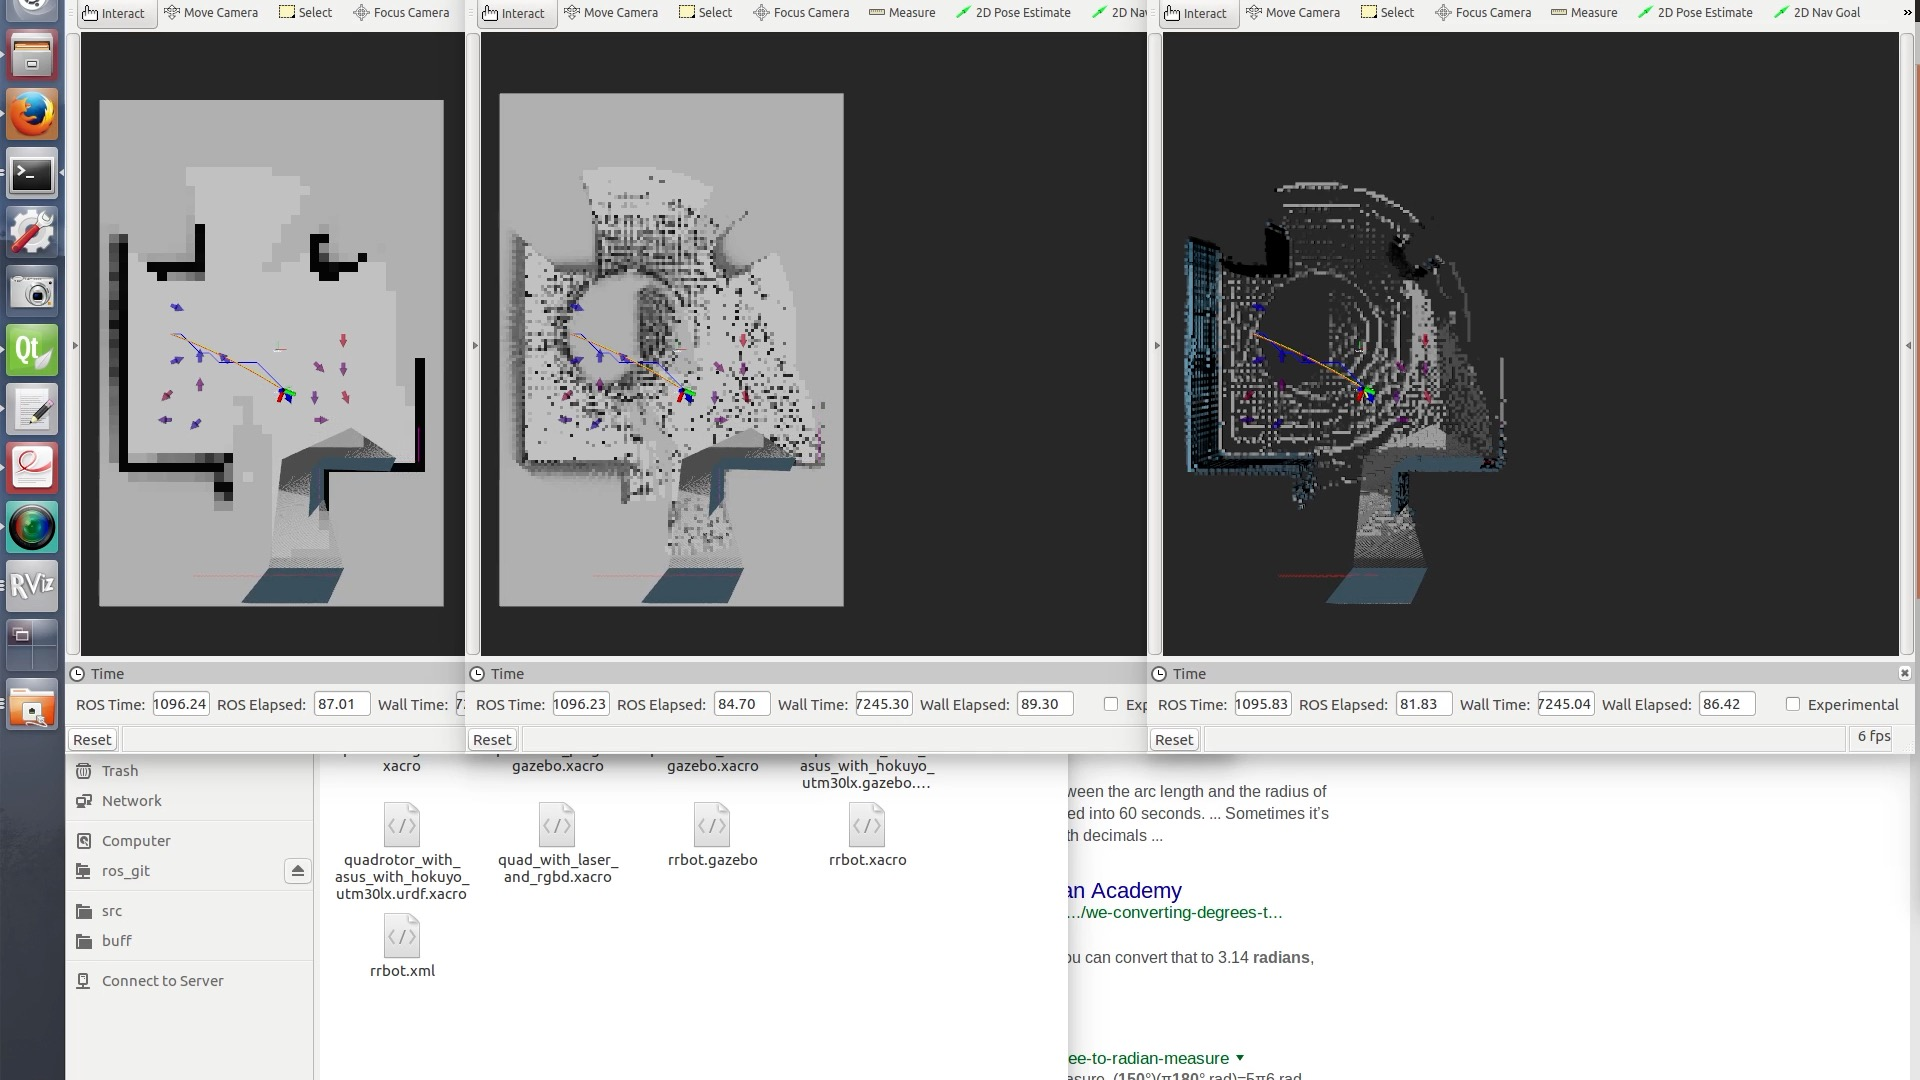
\includegraphics[trim = {41.5cm 17cm 14.3cm 3.8cm}, clip, height=\textwidth]{gazebo_1min.jpg}
        		\caption{$t=1$min}
    	\end{subfigure}
    	\begin{subfigure}[t]{0.24\columnwidth}
           	\centering
          	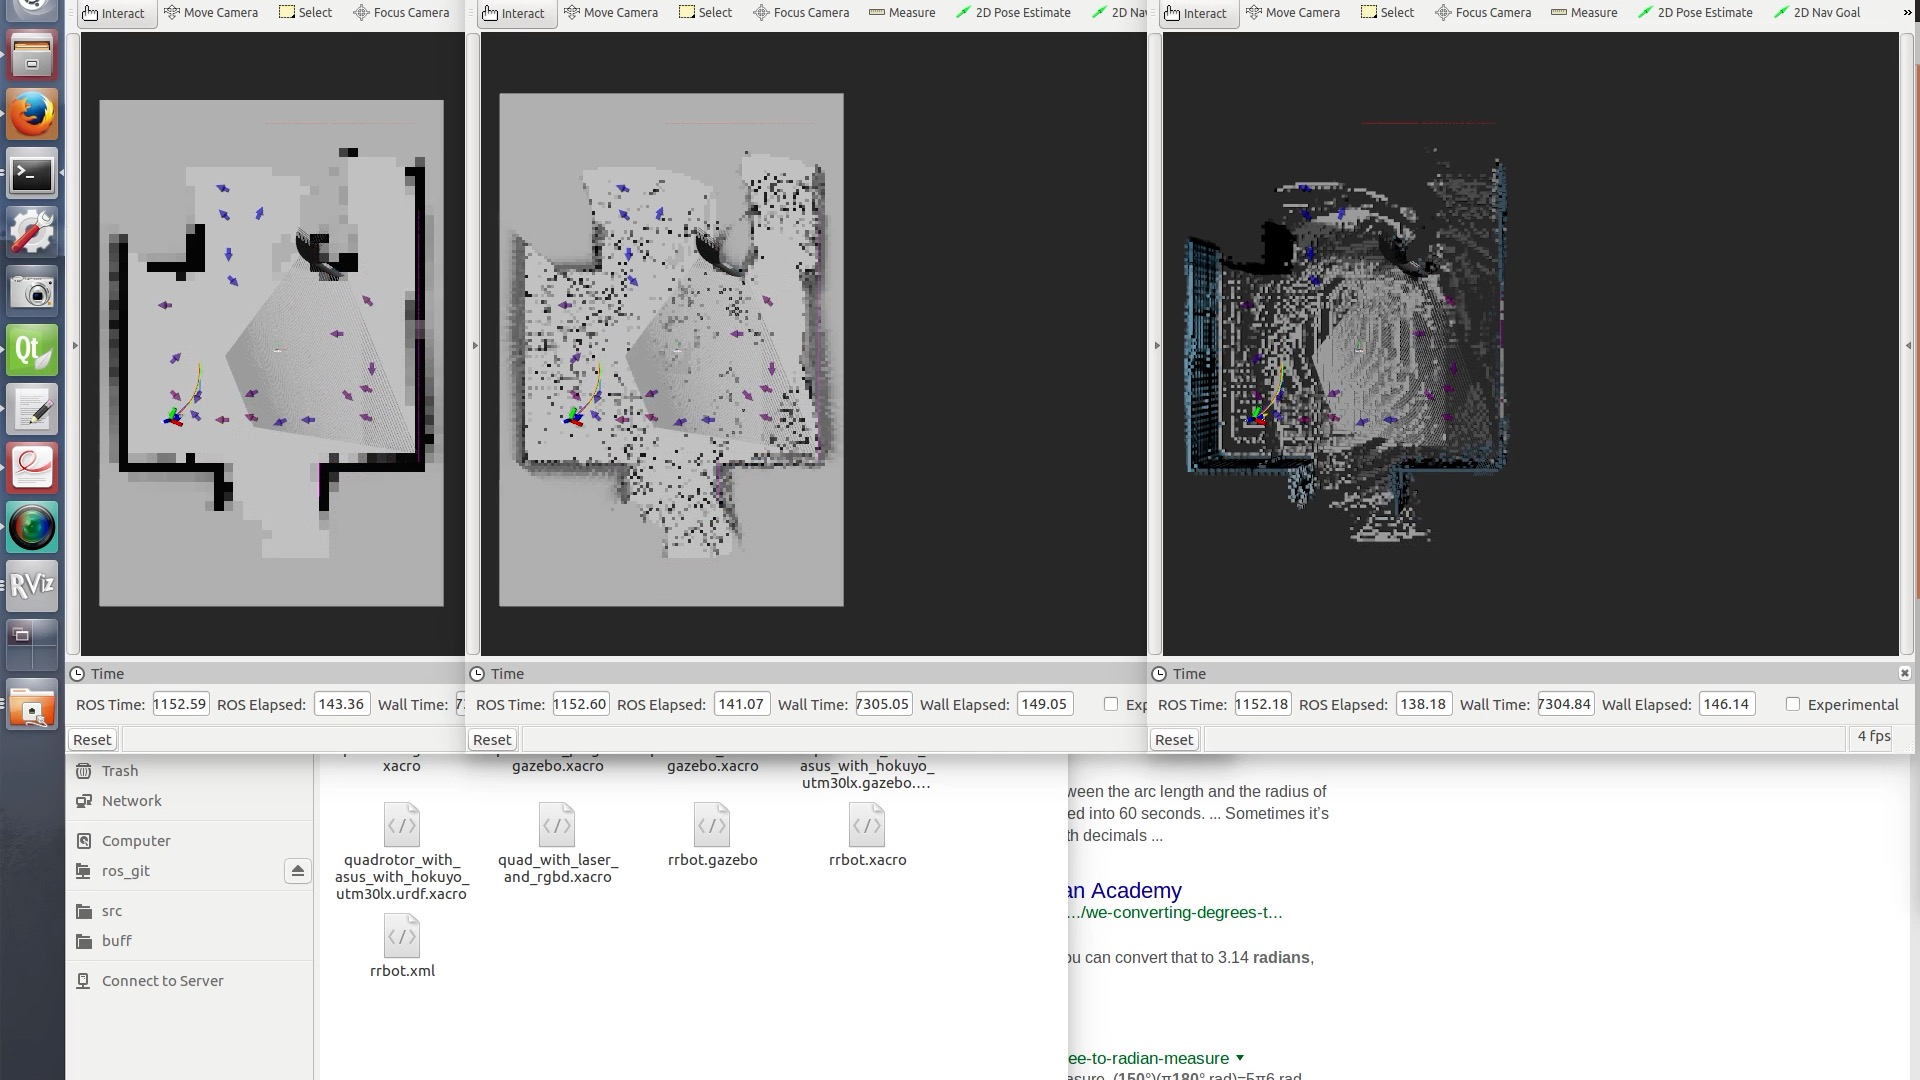
\includegraphics[trim = {41.5cm 17cm 14.3cm 3.8cm}, clip, height=\textwidth]{gazebo_2min.jpg}
        		\caption{$t=2$min}
    	\end{subfigure}
    	\begin{subfigure}[t]{0.24\columnwidth}
           	\centering
          	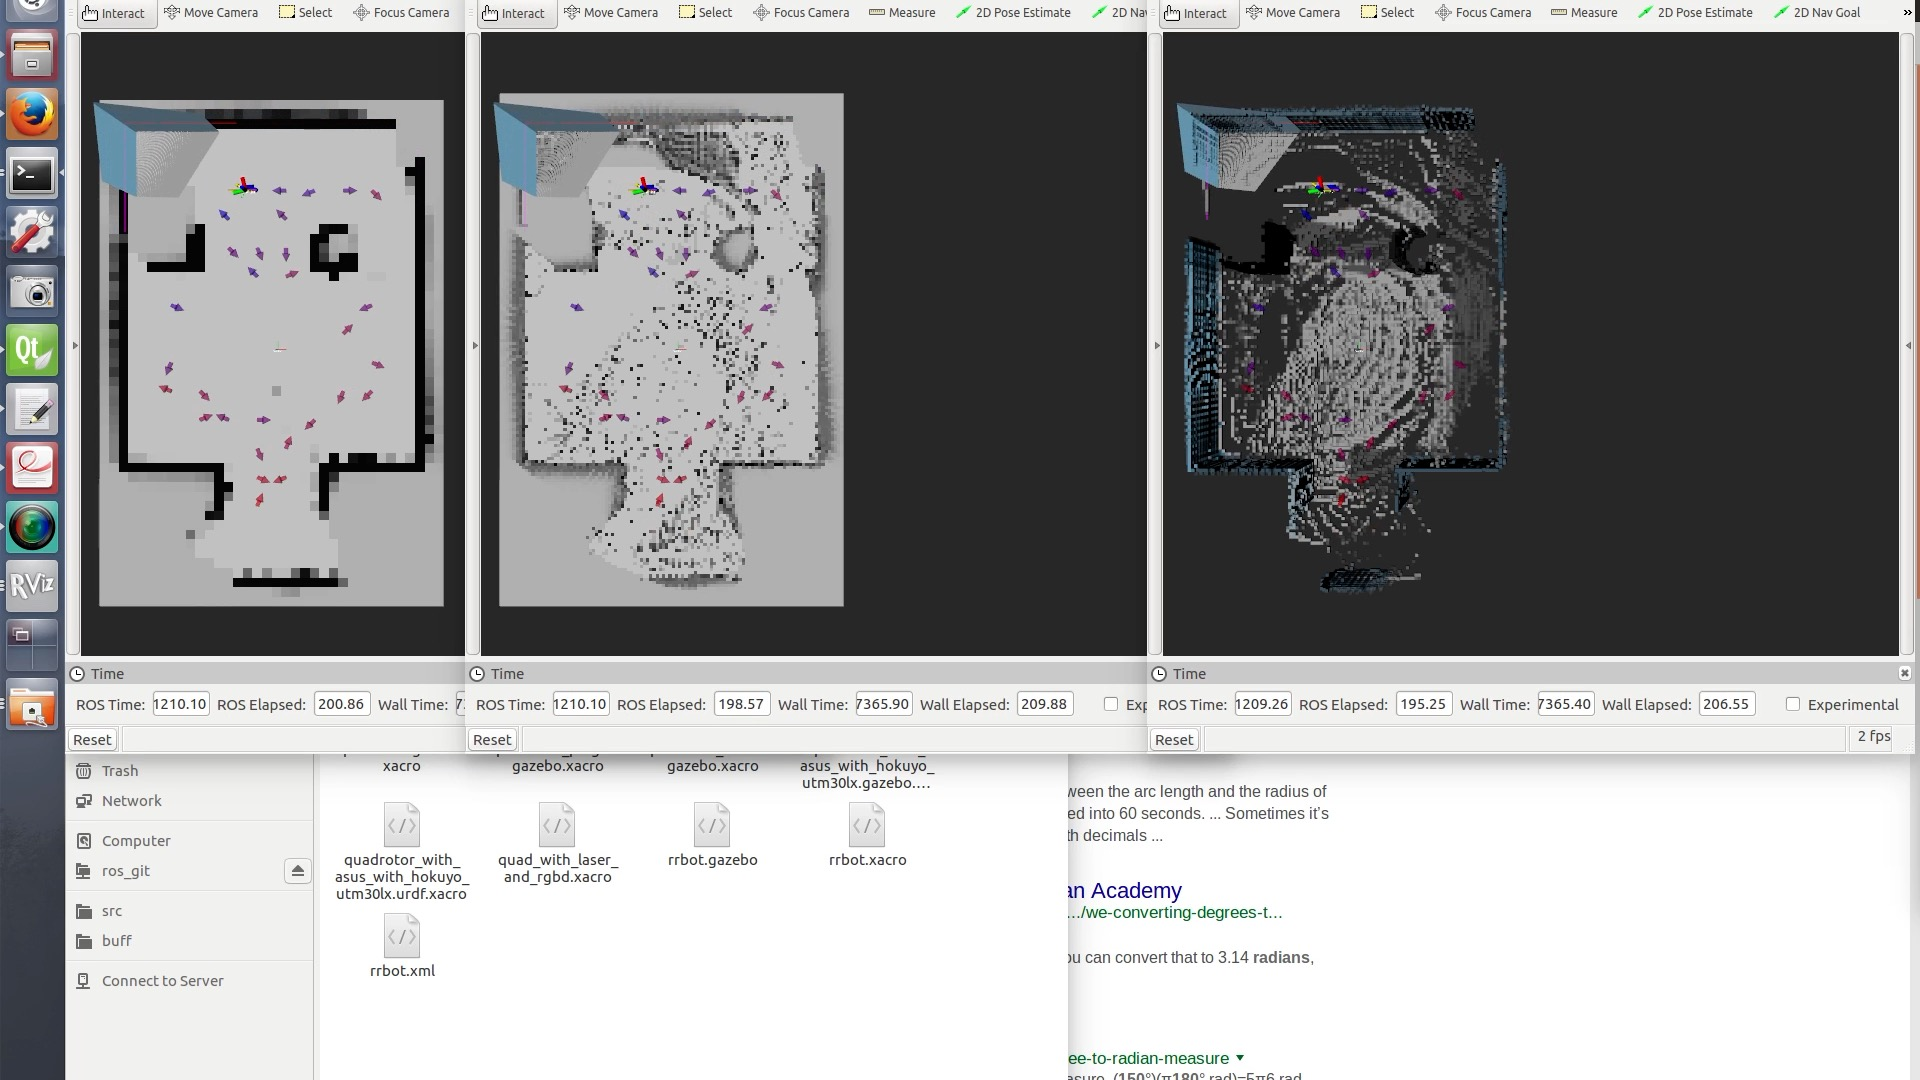
\includegraphics[trim = {41.5cm 17cm 14.3cm 3.8cm}, clip, height=\textwidth]{gazebo_3min.jpg}
        		\caption{$t=3$min}
   	\end{subfigure}
    	\begin{subfigure}[t]{0.24\columnwidth}
           	\centering
          	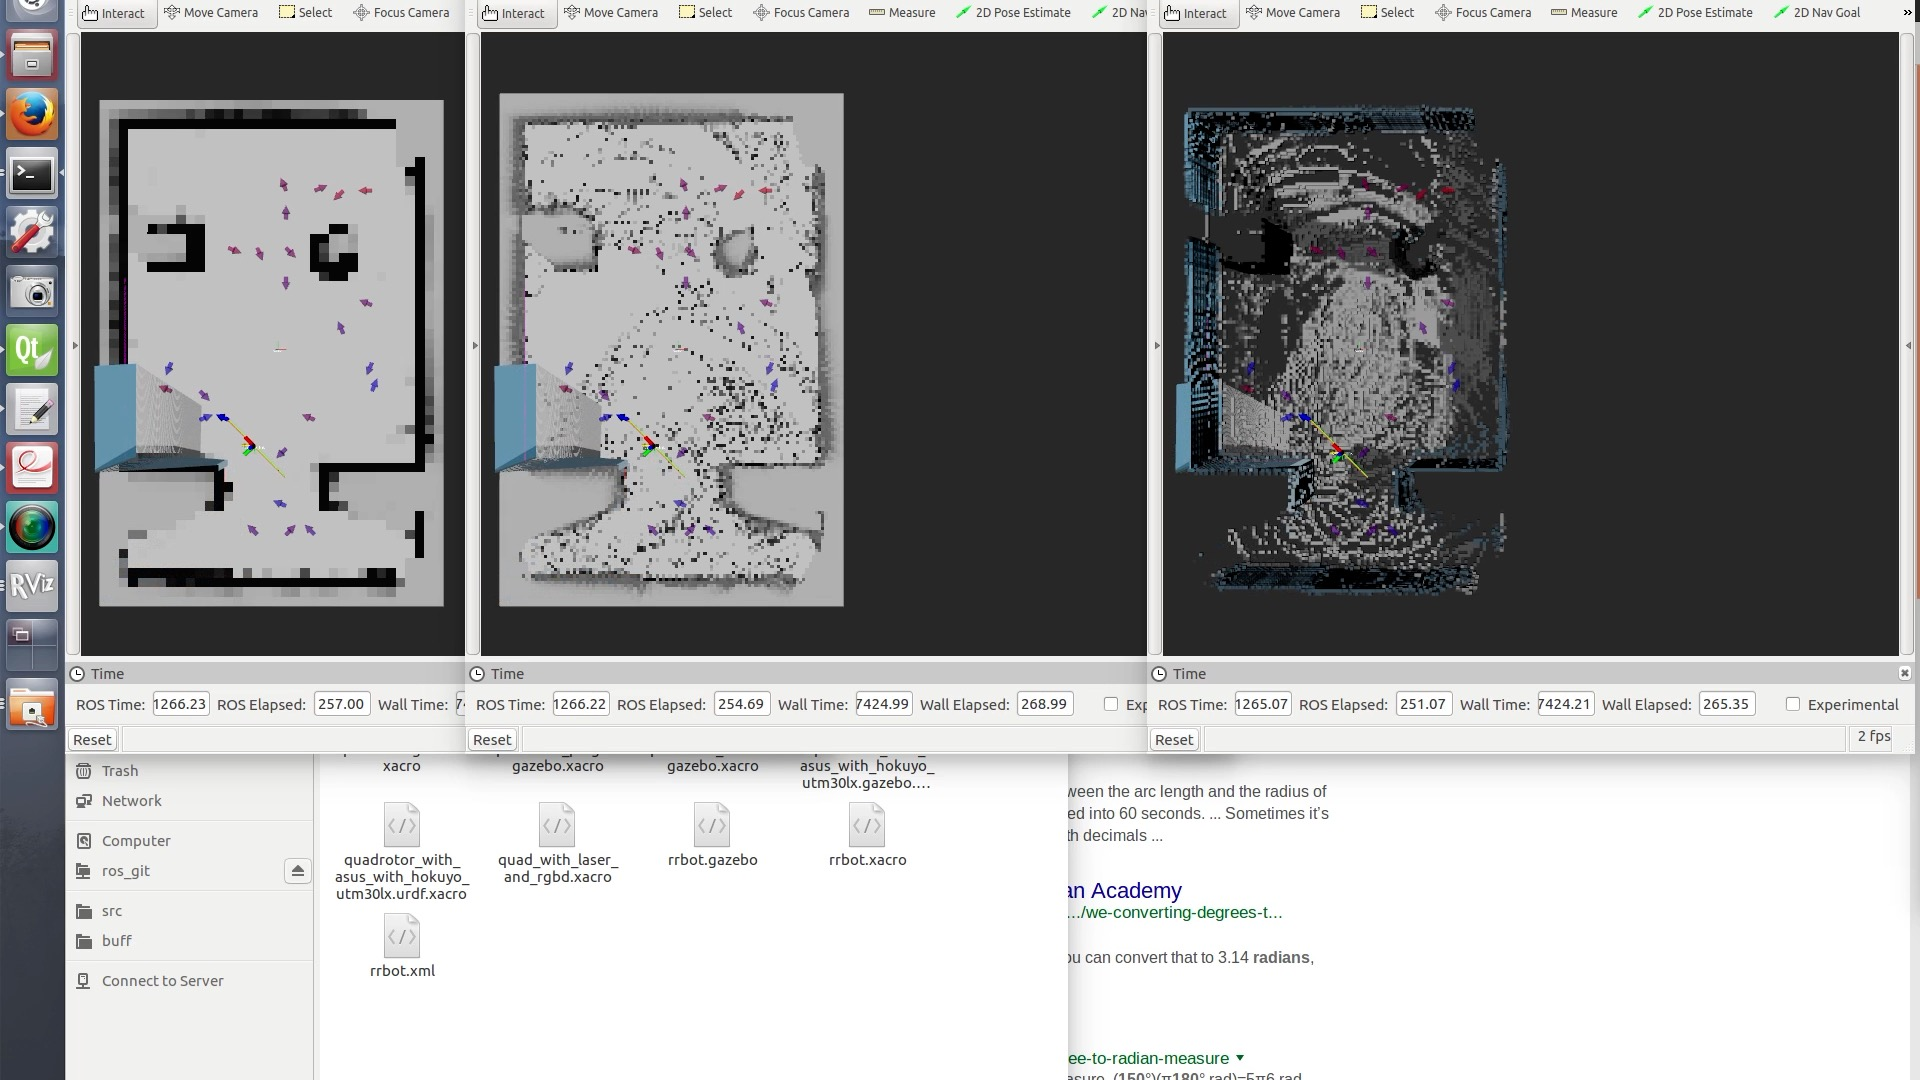
\includegraphics[trim = {41.5cm 17cm 14.3cm 3.8cm}, clip, height=\textwidth]{gazebo_4min.jpg}
        		\caption{$t=4$min}
    	\end{subfigure}
	\begin{subfigure}[t]{0.24\columnwidth}
           	\centering
          	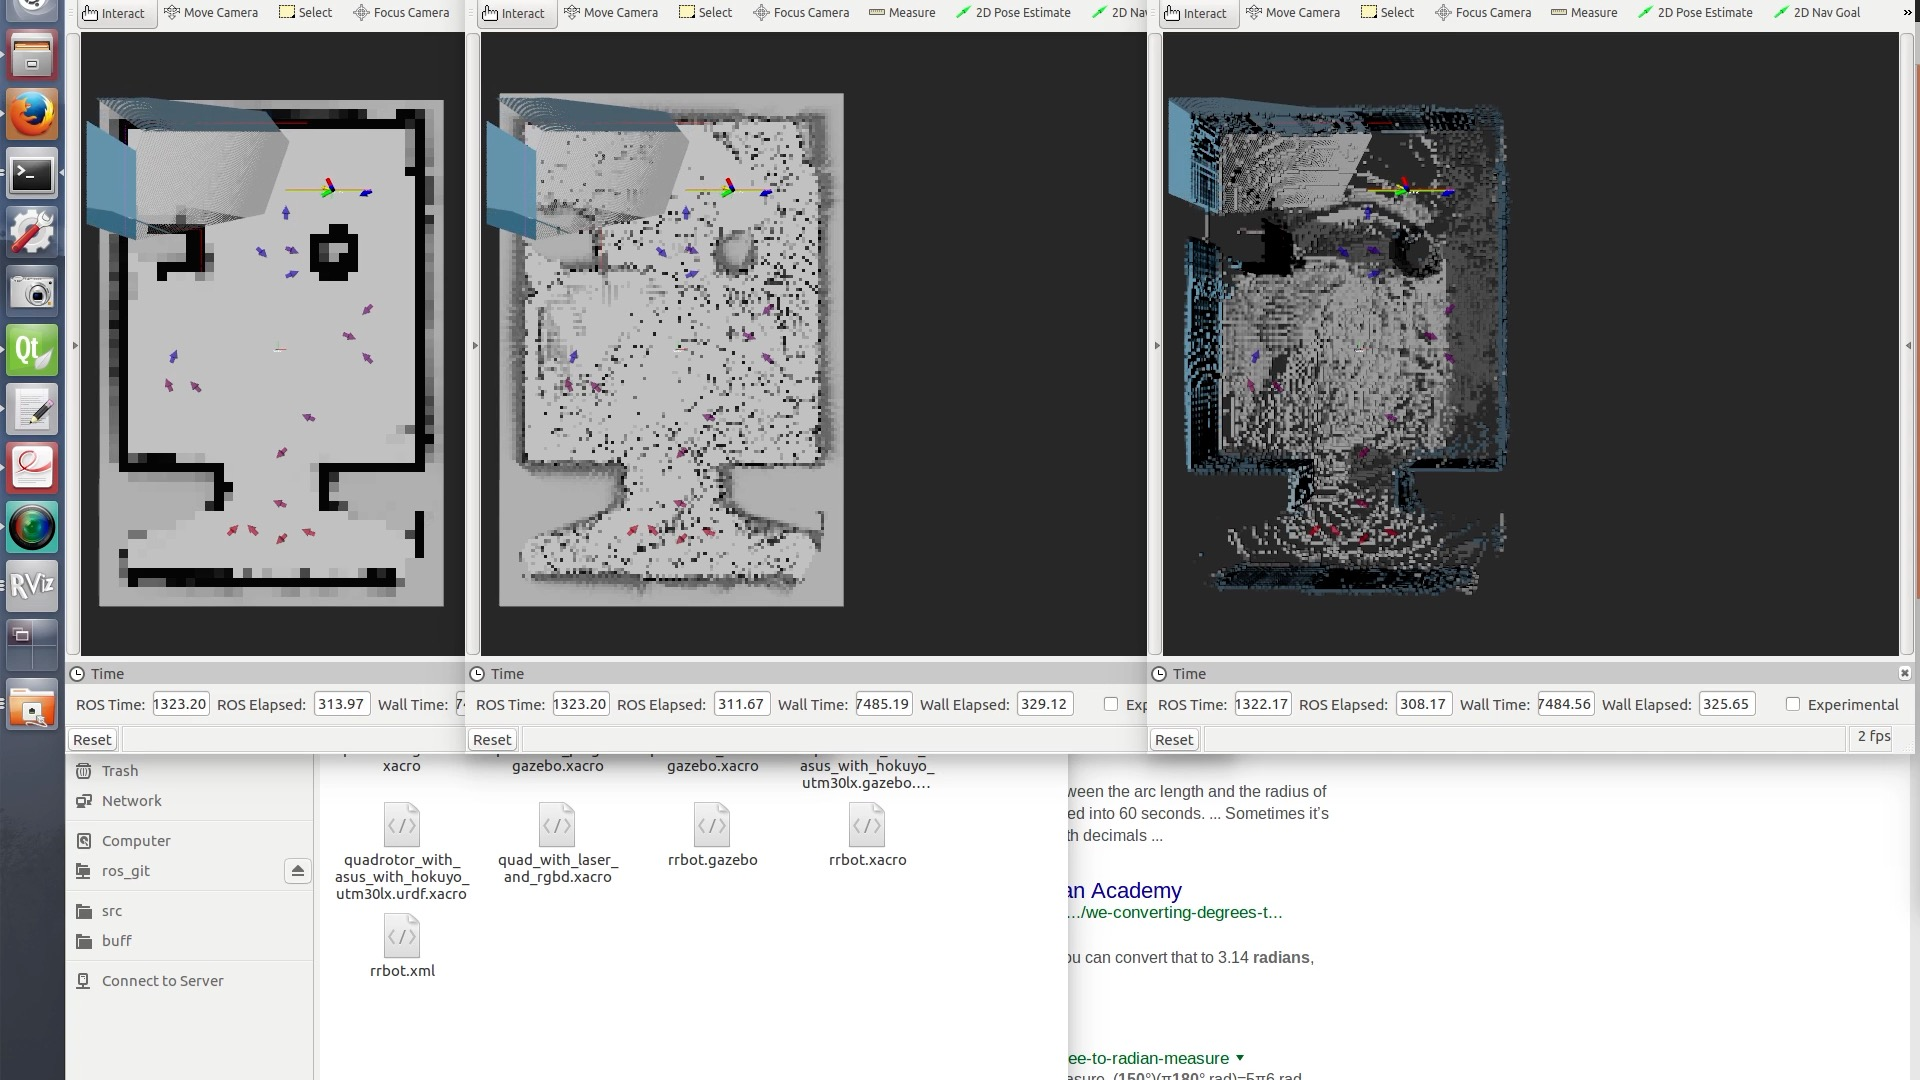
\includegraphics[trim = {41.5cm 17cm 14.3cm 3.8cm}, clip, height=\textwidth]{gazebo_5min.jpg}
        		\caption{$t=5$min}
    	\end{subfigure}
    	\begin{subfigure}[t]{0.24\columnwidth}
           	\centering
          	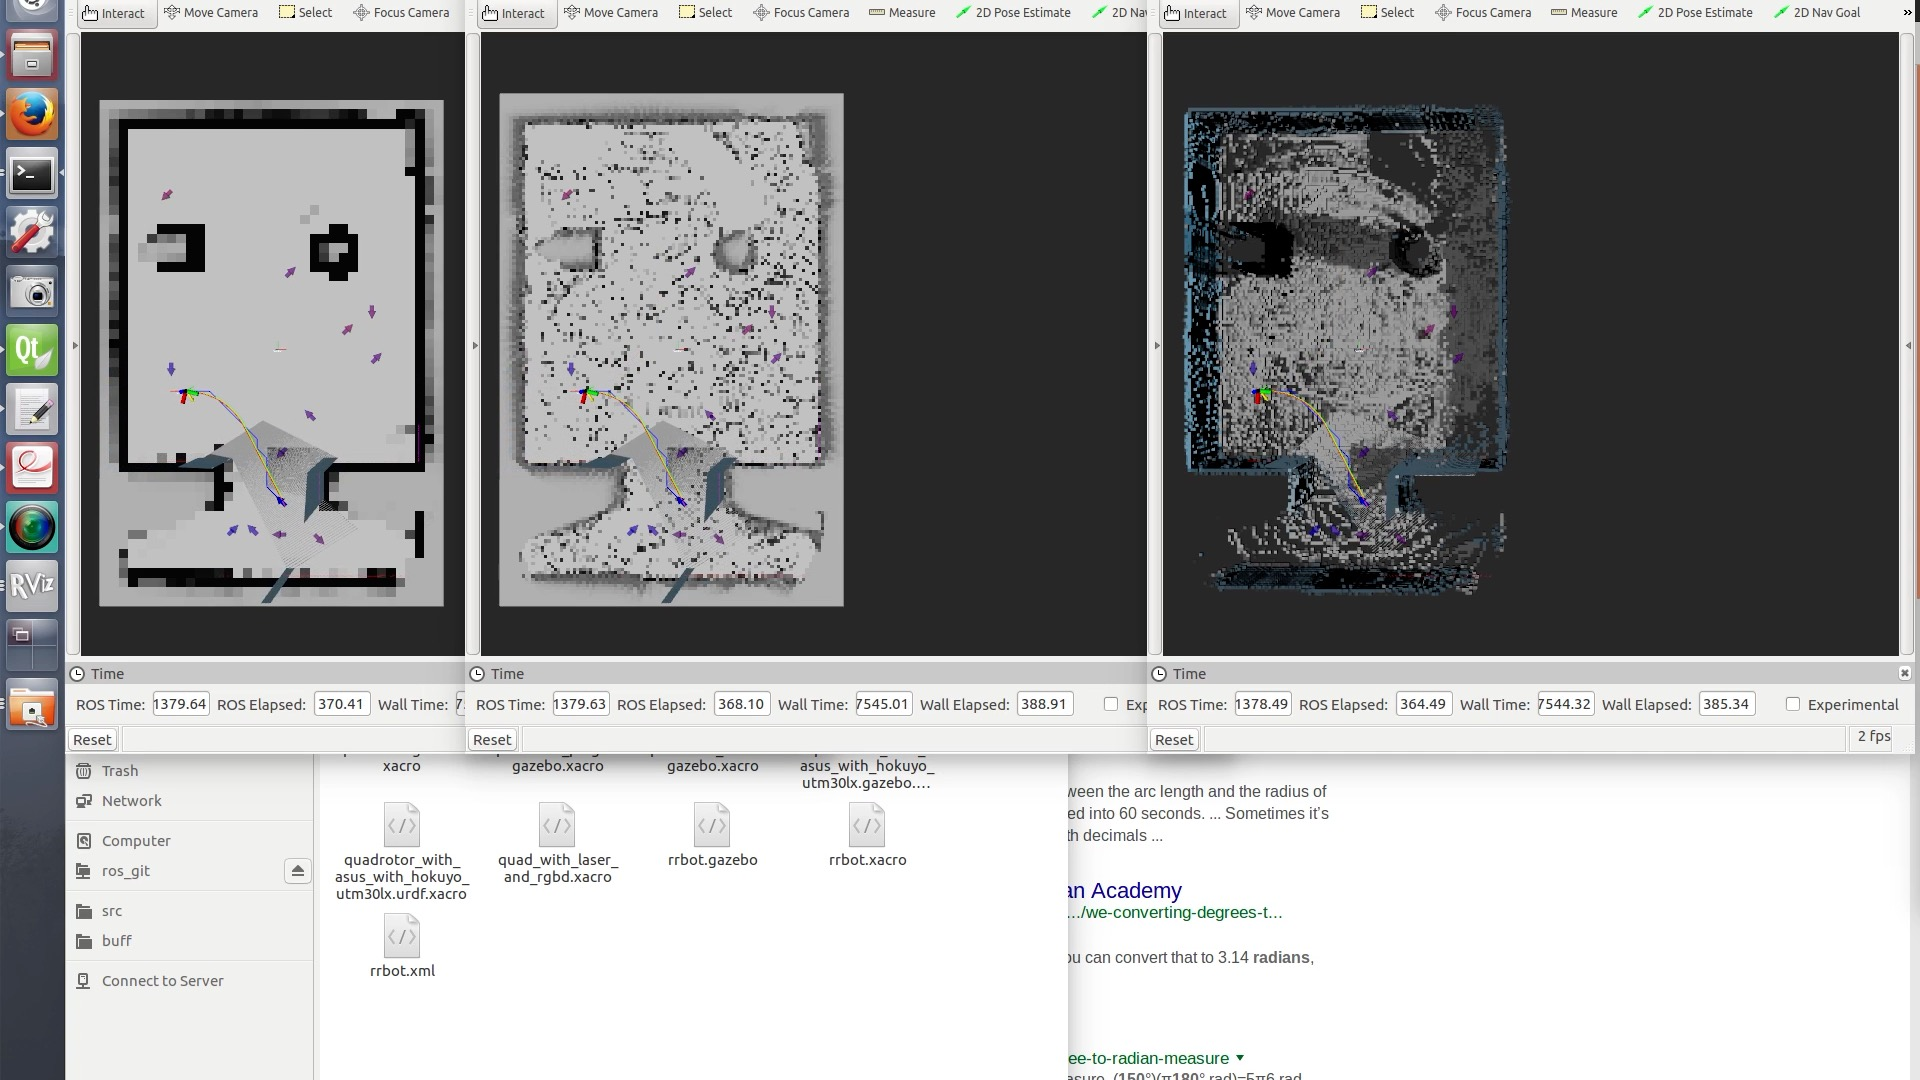
\includegraphics[trim = {41.5cm 17cm 14.3cm 3.8cm}, clip, height=\textwidth]{gazebo_6min.jpg}
        		\caption{$t=6$min}
    	\end{subfigure}
    	\begin{subfigure}[t]{0.24\columnwidth}
           	\centering
          	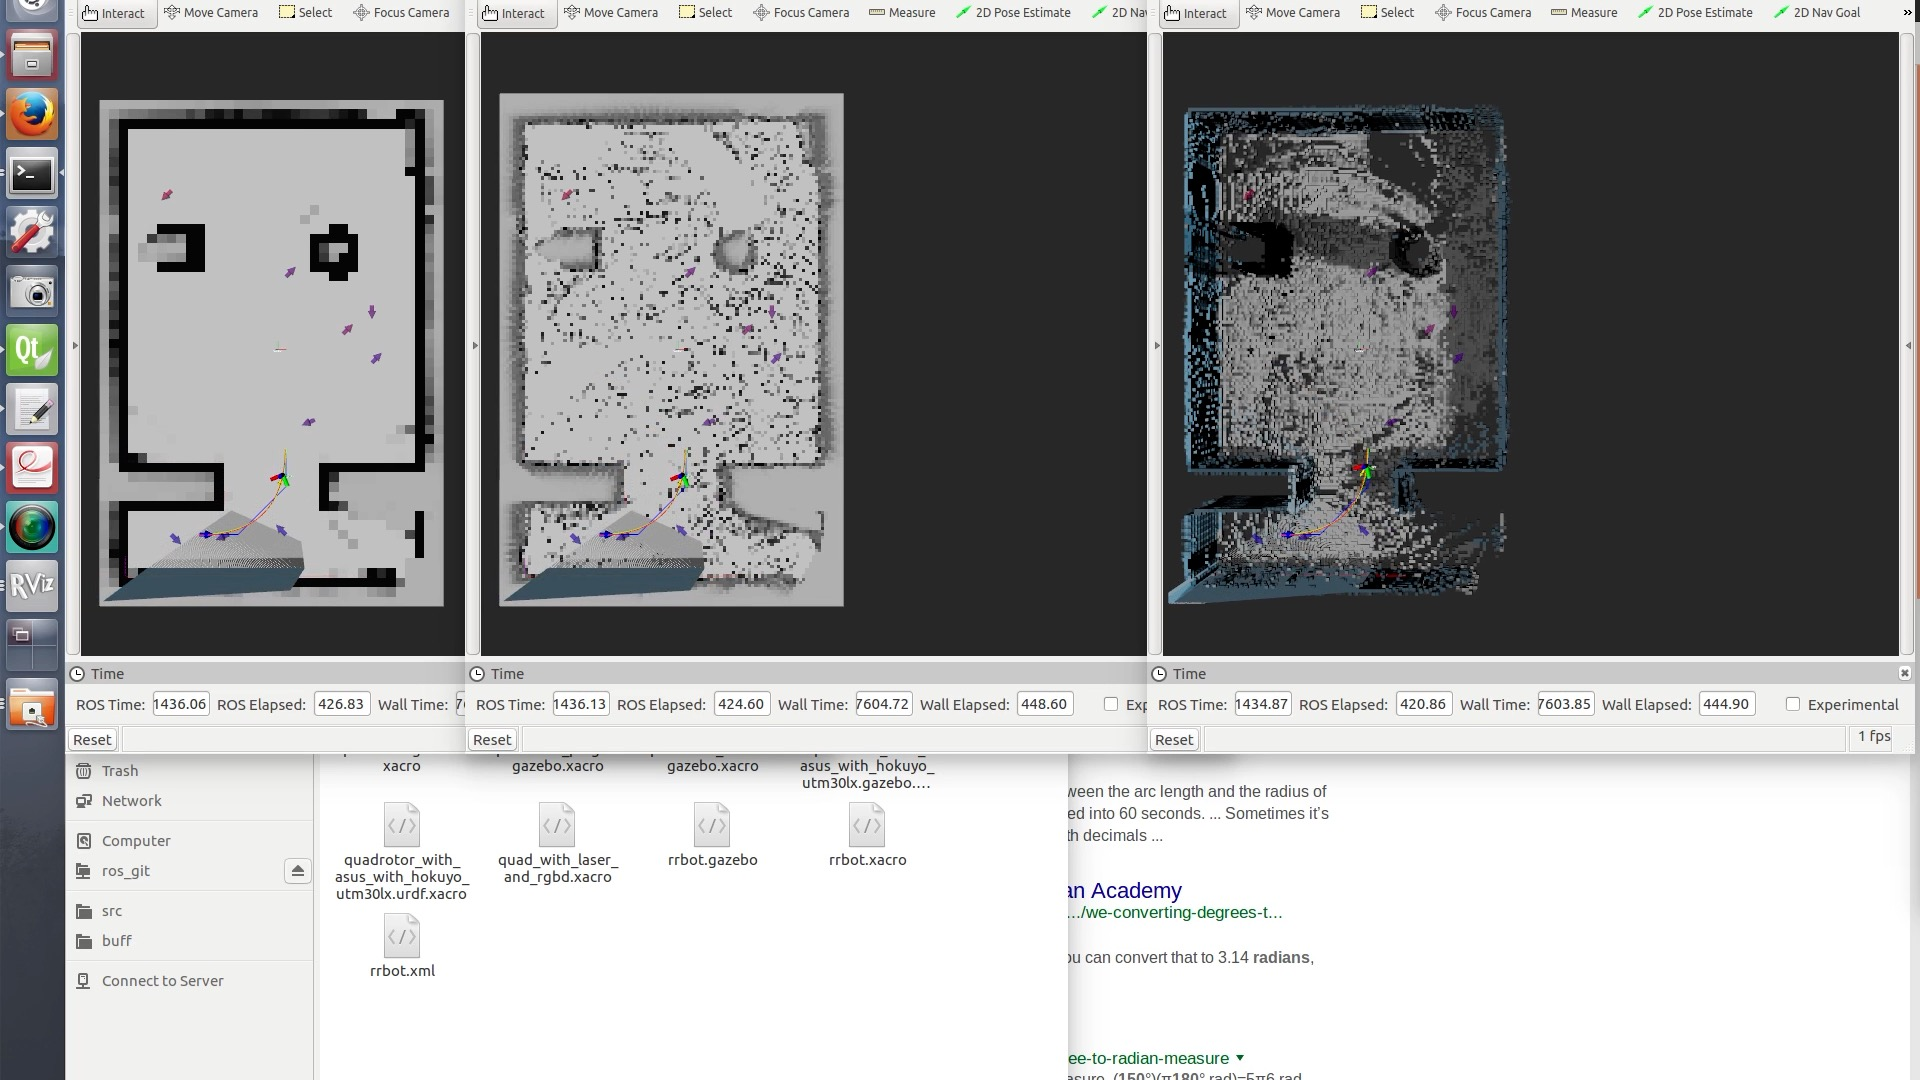
\includegraphics[trim = {41.5cm 17cm 14.3cm 3.8cm}, clip, height=\textwidth]{gazebo_7min.jpg}
        		\caption{$t=7$min}
   	\end{subfigure}
    	\begin{subfigure}[t]{0.24\columnwidth}
           	\centering
          	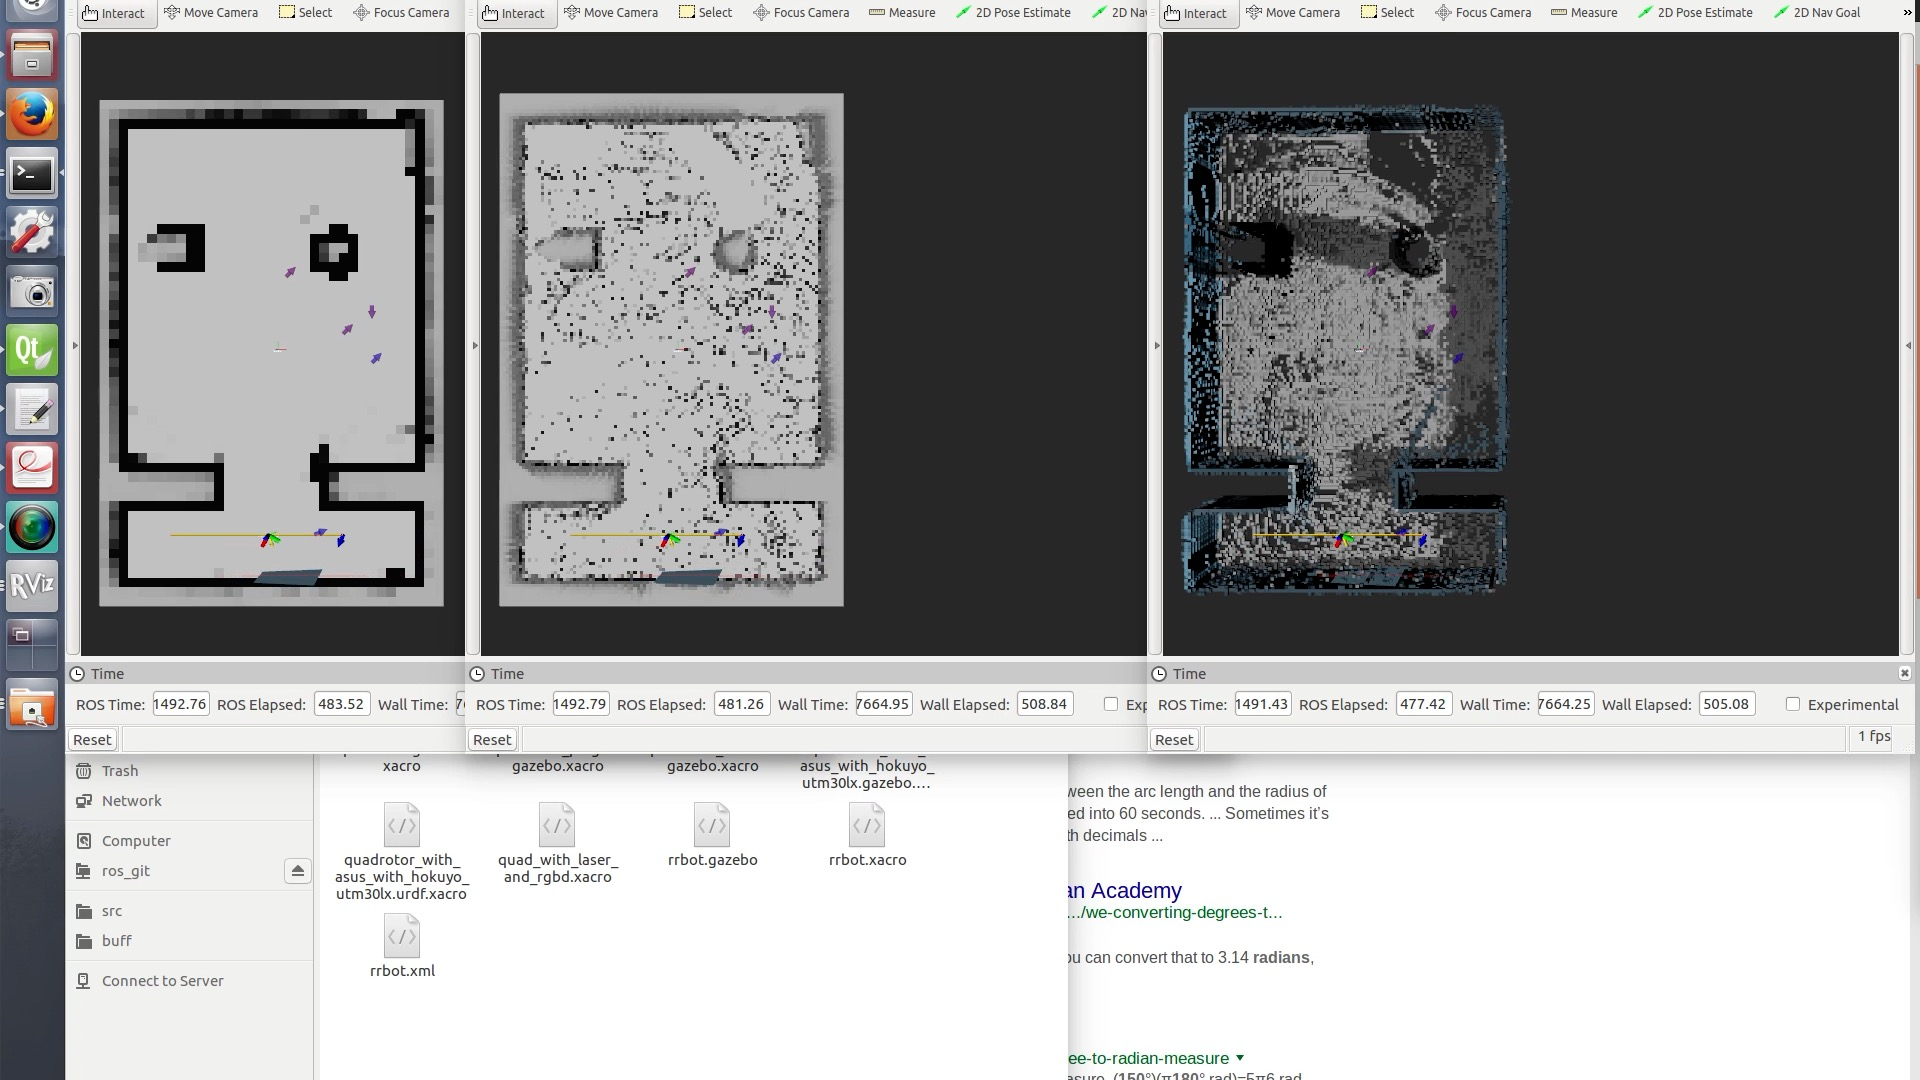
\includegraphics[trim = {41.5cm 17cm 14.3cm 3.8cm}, clip, height=\textwidth]{gazebo_8min.jpg}
        		\caption{$t=8$min}
    	\end{subfigure}
%\includegraphics[width=2.5in]{myfigure}
% where an .eps filename suffix will be assumed under latex, 
% and a .pdf suffix will be assumed for pdflatex; or what has been declared
% via \DeclareGraphicsExtensions.
\caption{Simulated 3D Occupancy Grid Map}
\label{fig:sim3DMap}
\end{figure}


\begin{figure}[!t]
	\centering
	\begin{subfigure}[t]{0.3\columnwidth}
           	\centering
          	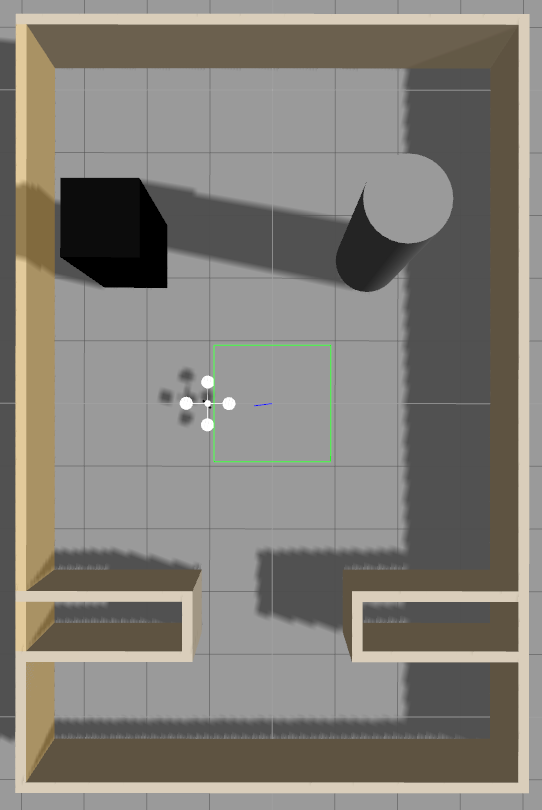
\includegraphics[height=1.5\textwidth]{gazebo_view.png}
        		\caption{Environment}
    	\end{subfigure}
		\hspace*{0.05cm}
    	\begin{subfigure}[t]{0.3\columnwidth}
           	\centering
          	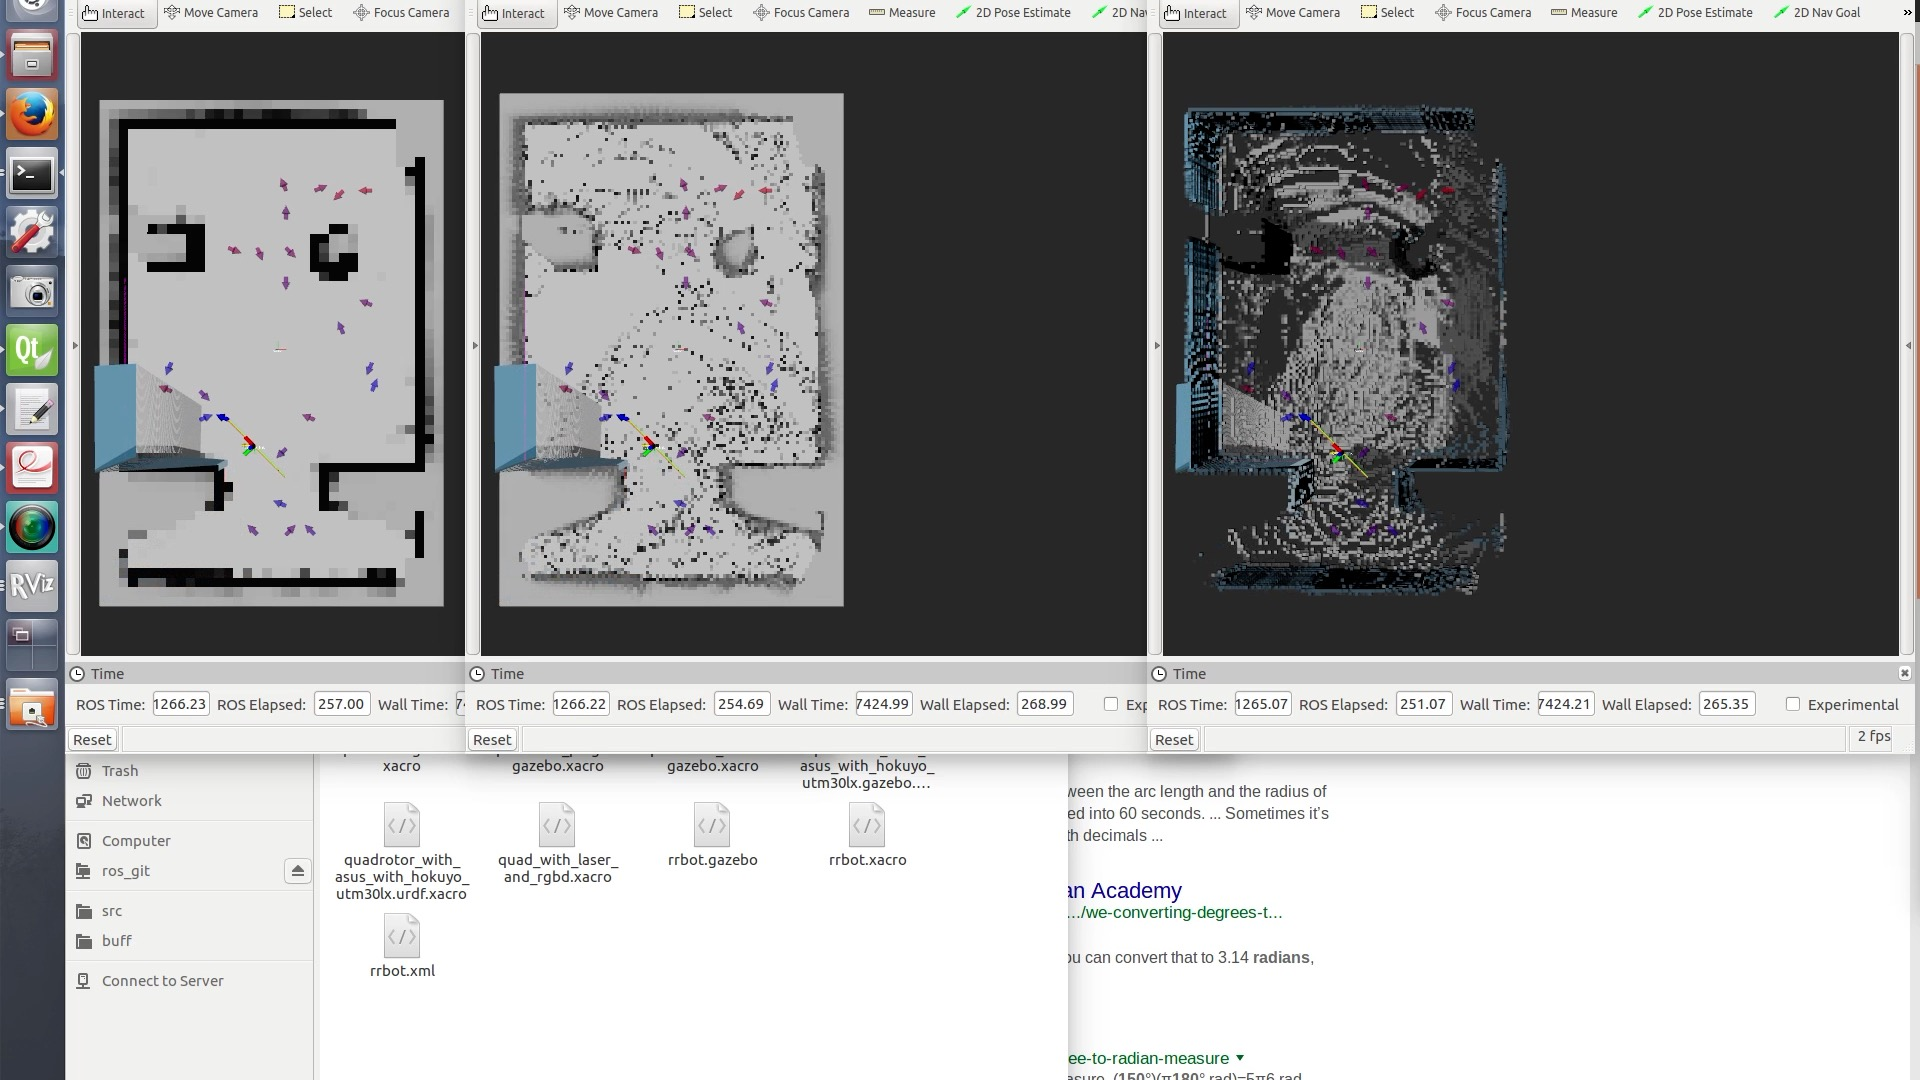
\includegraphics[trim = {3.6cm 17cm 52.5cm 4cm}, clip, height=1.5\textwidth]{gazebo_4min.jpg}
        		\caption{Collision Map}
    	\end{subfigure}
	\hspace*{0.1cm}
	\begin{subfigure}[t]{0.3\columnwidth}
           	\centering
          	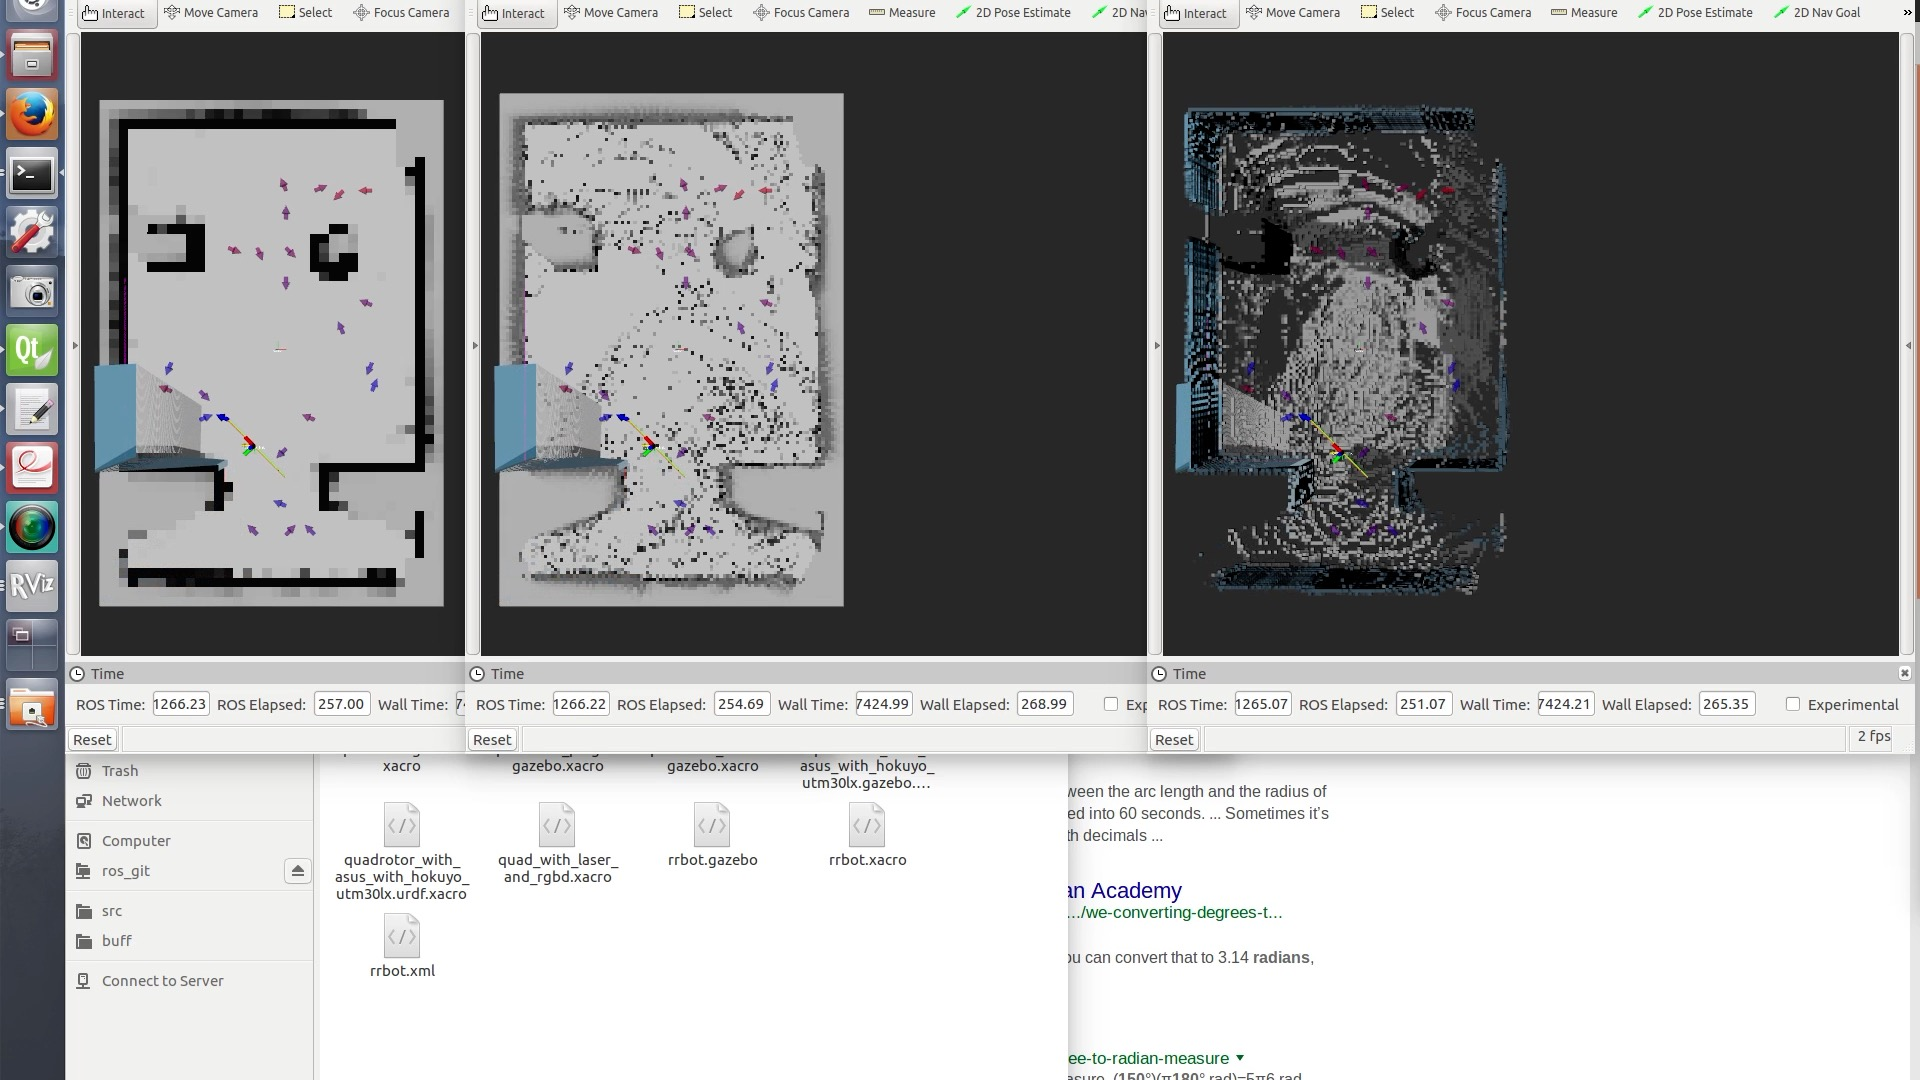
\includegraphics[trim = {18cm 17cm 38.1cm 4cm}, clip, height=1.5\textwidth]{gazebo_4min.jpg}
        		\caption{Entropy Map}
    	\end{subfigure}
%\includegraphics[width=2.5in]{myfigure}
% where an .eps filename suffix will be assumed under latex, 
% and a .pdf suffix will be assumed for pdflatex; or what has been declared
% via \DeclareGraphicsExtensions.
\caption{Simulated Environment and 2D Projected Maps at $4$min}
\label{fig:sim2Dmaps}
\end{figure}

\begin{figure}[!t]
	\centering
	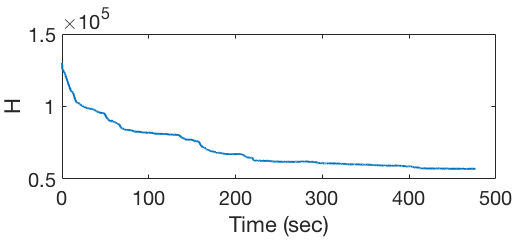
\includegraphics[width=0.4\textwidth]{entropy_gazebo_aspect3by1.png}
	\caption{Simulated Environment Map Entropy}
	\label{fig:simH}
\end{figure}

The two-map approach exhibits advantages and disadvantages. The exploration algorithm successfully avoided collisions and gave way to a fairly complete 3D occupancy grid. The floor, which is not always visible, is properly estimated in most places. Conversely, this attention to detail has negative consequences that encourage the robot to repeatedly look at the same regions from different vantage points.
Since an entropy map cell is composed from many 3D grid cells single-stacked vertically, if just one of these 3D map cells is not captured or hardly captured, the entropy map cell will be recorded as quite uncertain, shown covering numerous locations in Fig. \ref{fig:sim2Dmaps}(c). The robot may attempt to measure this space again, even when other regions might more strongly warrant observation. These periods of sluggish entropy decrease are shown with flatter sections of Fig. \ref{fig:simH}. In short, this algorithm successfully explores the space collision-free while producing a complete map, but over-attention to just a few uncertain cells has negative consequences on the exploration speed.


\section{Experimental Resutls}

\subsection{Exploration Environment}

The Laboratory for Autonomous Systems Research (LASR) at the U.S. Naval Research Laboratory (NRL) provides a large experimental space for testing. An experimental setup resembles a building floor plan, which involves tan cardboard suspended from $1$m tall stanchions for a perimeter wall, an internal wall from $80/20$ supports with grey sheeting inside, and a floor that reflects some of the florescent lights above. Additionally, there are two wooden table desks with chairs and miscellaneous objects on top, and three plastic trash cans of varying sizes and colors. The map limits are designed to slightly exceed the experimental space: $0.5$m to $10.3$m in the x-direction (positive east), $-8.3$m to $3.5$m in the y-direction (positive north), and $-0.15$m to $1.5$m in the z-direction (positive vertically up). Pictures of the environment are shown in Fig. \ref{fig:exp3DEnvironment}.

\begin{figure}[!t]
\centering
    	\begin{subfigure}[t]{0.44\columnwidth}
           	\centering
          	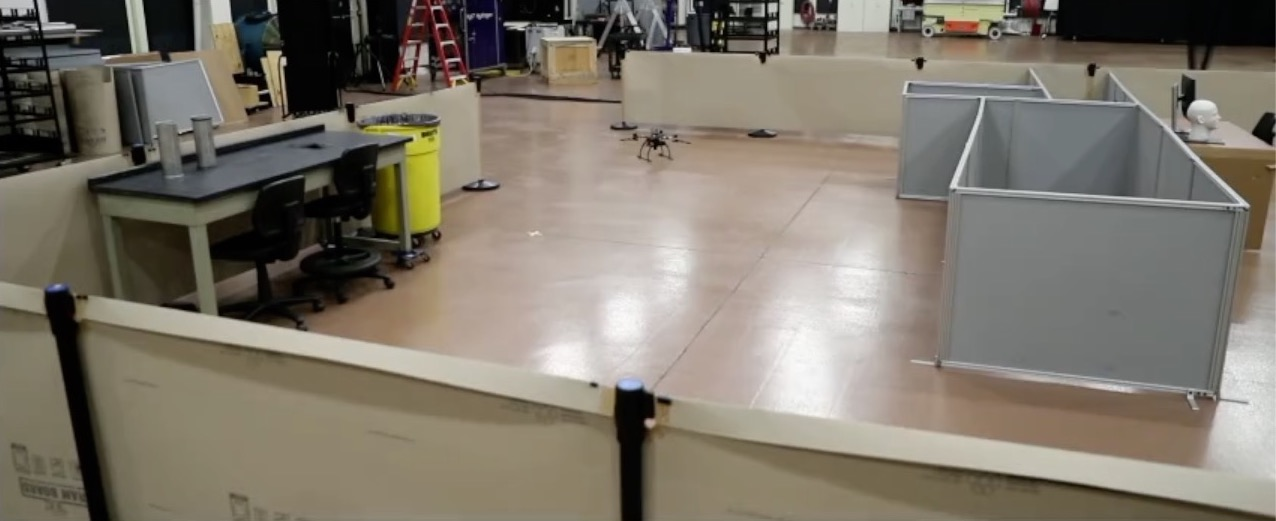
\includegraphics[width=\textwidth]{experiment_north.jpg}
        		\caption{North Region}
    	\end{subfigure}
    	\begin{subfigure}[t]{0.44\columnwidth}
           	\centering
          	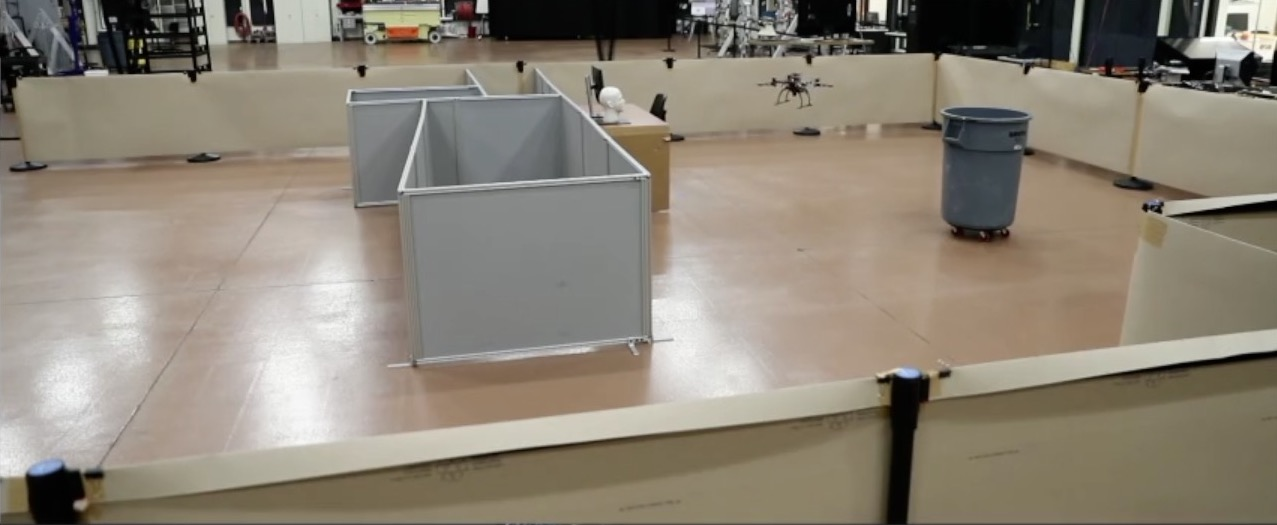
\includegraphics[width=\textwidth]{experiment_south.jpg}
        		\caption{South Region}
    	\end{subfigure}
	\caption{3D Experimental Environment}
	\label{fig:exp3DEnvironment}
\end{figure}


%        A.      Exploration Environment
%                perhaps adding size, feature and materials

\subsection{Hardware Structure}
%        B.      Hardware Structure

Instead of using a simulated environment such as Gazebo, where the robot state can be set and measured directly, a Vicon motion capture system produces pose data used in mapping and exploration transforms. An Asus Xtion and Hokuyo LIDAR are streamed from an onboard NVidia Jetson TX2 via Wifi to a host computer running the mapping and exploration nodes with an Intel Core i7-6800K CPU (12$\times$3.40GHz). The exploration trajectories are sent back to the Jetson TX2 over Wifi, where a nonlinear geometric flight controller~\cite{GooDaeLee13} is run onboard the Jetson to follow these trajectories. This configuration avoids large processing tasks onboard the robot.


\subsection{Experimental Results}
%        C.      Experiments Results
%                a little bit more interpretations and figures for the results
                
The experimental setup follows similar conditions as the simulated results with a few key differences. Most importantly, the second proposed exploration approach, namely a collision and entropy combination map, replaces the two-map approach used in simulation. The resulting 3D maps at various time steps are shown in Fig. \ref{fig:exp3DMap}. The 2D projected maps (x-direction upward) at corresponding time steps are illustrated in Figure \ref{fig:exp2DMap}, where trajectories are shown with curves to candidate poses are shown with arrows. The total map entropy as a function of time is shown in Figure \ref{fig:expH}.

% trim={<left> <lower> <right> <upper>}

\begin{figure}[!t]
\centering
    	\begin{subfigure}[t]{0.88\columnwidth}
           	\centering
          	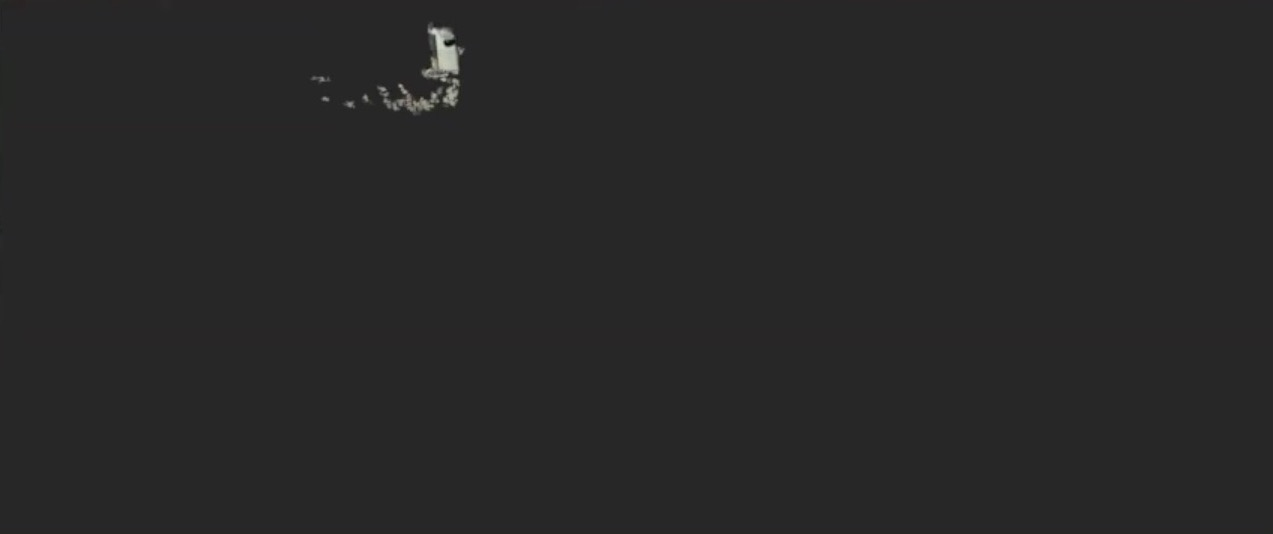
\includegraphics[width=\textwidth]{experiment_ogm3D_0min.jpg}
        		\caption{$0$min}
    	\end{subfigure}
    	\begin{subfigure}[t]{0.88\columnwidth}
           	\centering
          	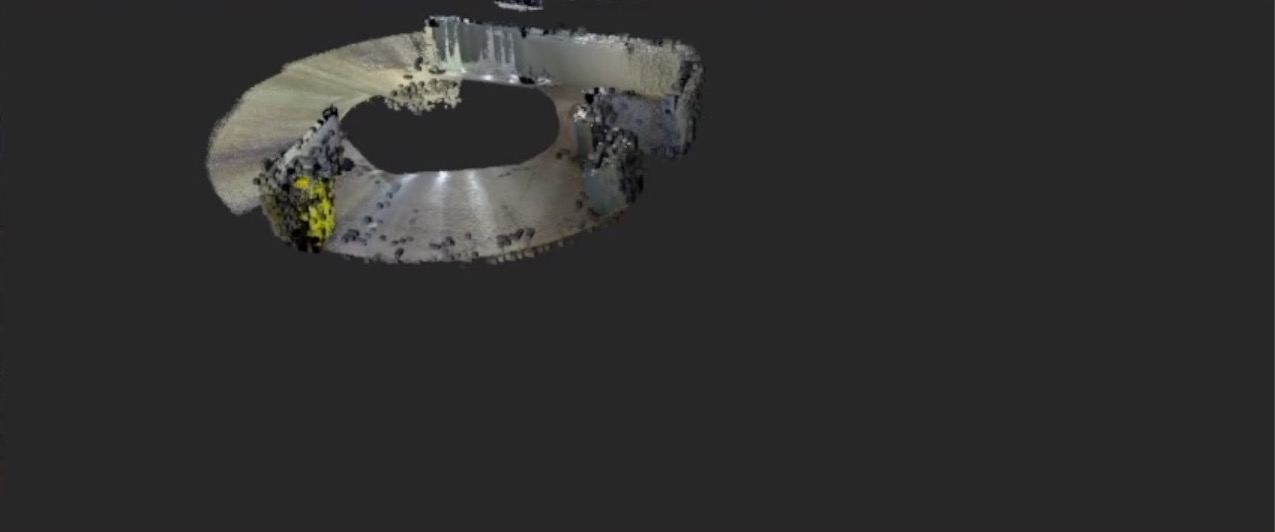
\includegraphics[width=\textwidth]{experiment_ogm3D_1min.jpg}
        		\caption{$1$min}
    	\end{subfigure}
    	\begin{subfigure}[t]{0.88\columnwidth}
           	\centering
          	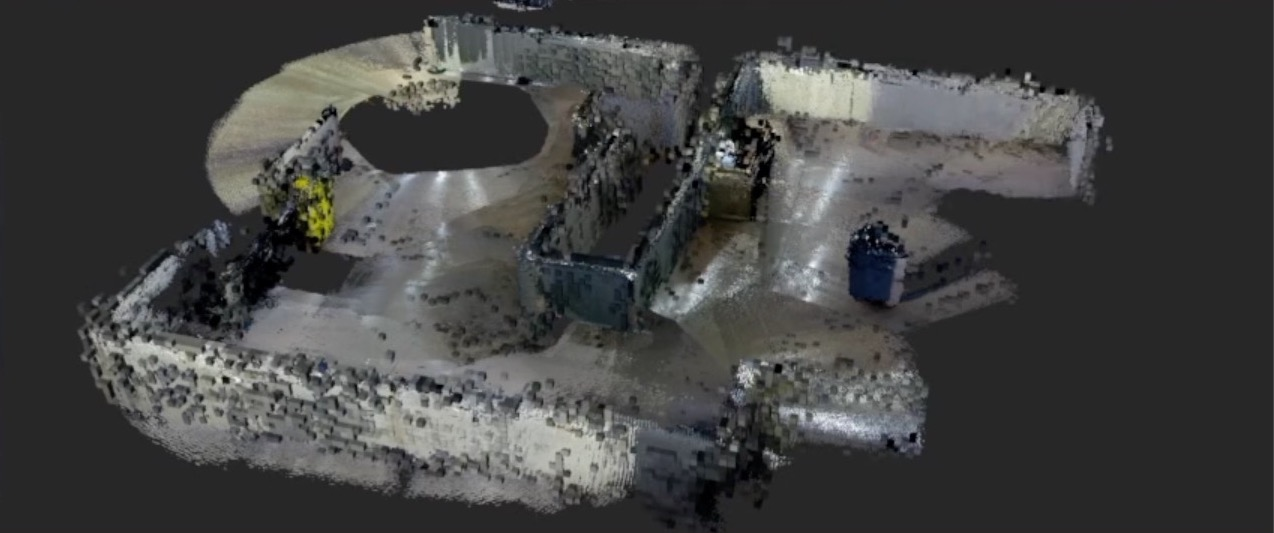
\includegraphics[width=\textwidth]{experiment_ogm3D_2min.jpg}
        		\caption{$2$min}
    	\end{subfigure}
    	\begin{subfigure}[t]{0.88\columnwidth}
           	\centering
          	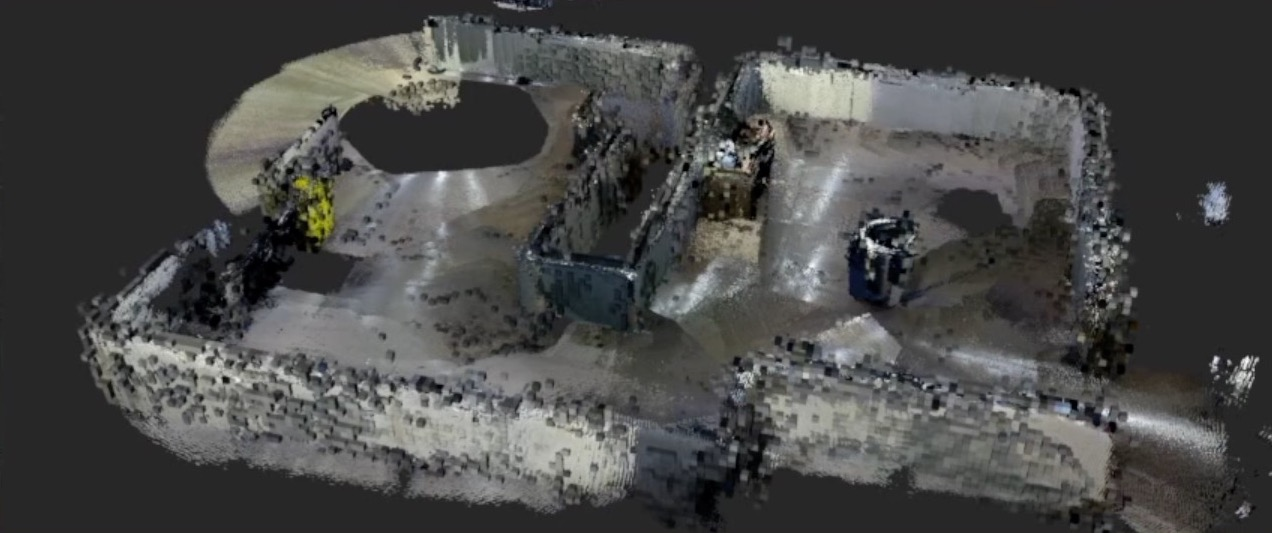
\includegraphics[width=\textwidth]{experiment_ogm3D_2min47sec.jpg}
        		\caption{$2$min $47$sec (end)}
    	\end{subfigure}
	\caption{3D Occupancy Grid Map and Point Clouds}
	\label{fig:exp3DMap}
\end{figure}

\begin{figure}[!t]
\centering
    	\begin{subfigure}[t]{0.44\columnwidth}
           	\centering
          	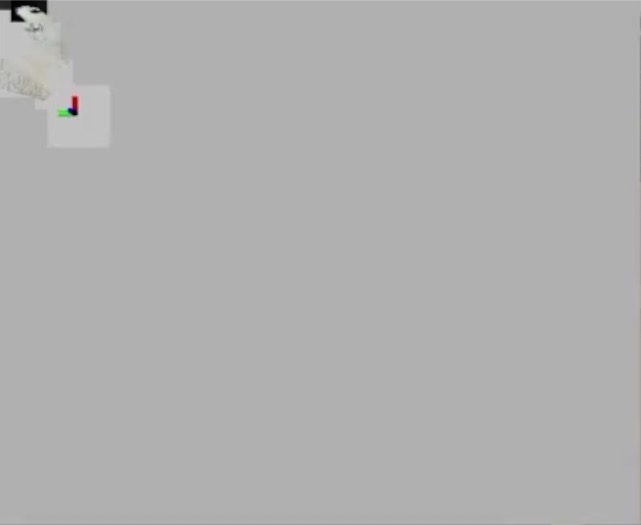
\includegraphics[width=\textwidth]{experiment_0min_2D.jpg}
        		\caption{$0$min}
    	\end{subfigure}
    	\begin{subfigure}[t]{0.44\columnwidth}
           	\centering
          	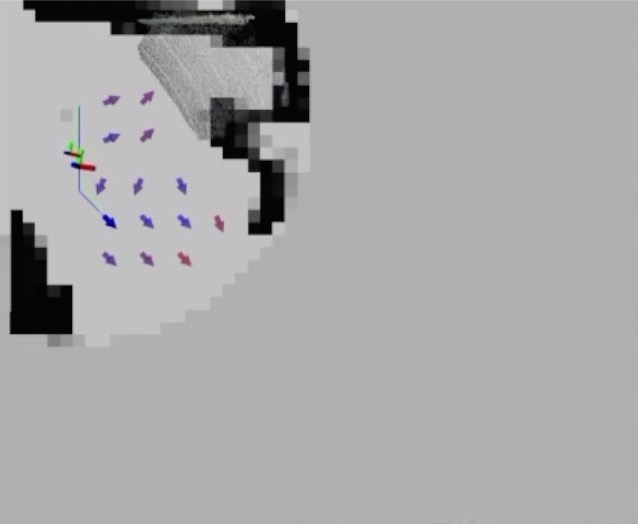
\includegraphics[width=\textwidth]{experiment_1min_2D.jpg}
        		\caption{$1$min}
    	\end{subfigure}
    	\begin{subfigure}[t]{0.44\columnwidth}
           	\centering
          	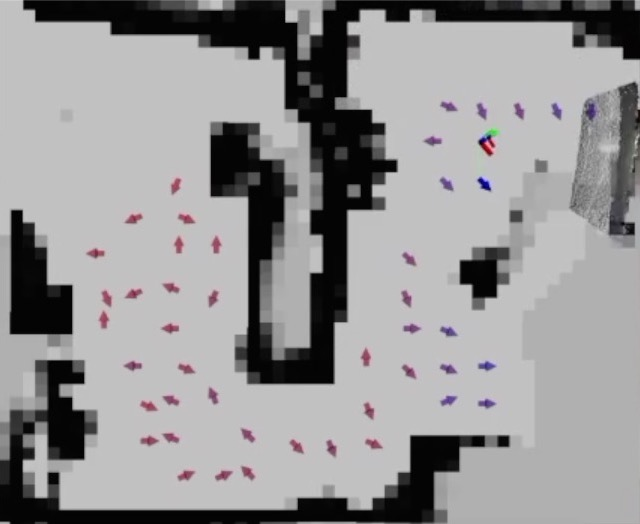
\includegraphics[width=\textwidth]{experiment_2min_2D.jpg}
        		\caption{$2$min}
    	\end{subfigure}
    	\begin{subfigure}[t]{0.44\columnwidth}
           	\centering
          	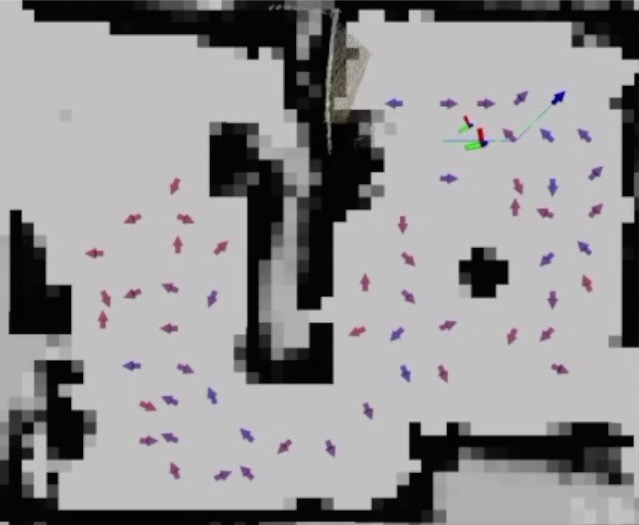
\includegraphics[width=\textwidth]{experiment_2min47sec_2D.jpg}
        		\caption{$2$min $47$sec (end)}
    	\end{subfigure}
	\caption{2D Collision and Exploration Combination Map}
	\label{fig:exp2DMap}
\end{figure}

\begin{figure}[!t]
	\centering
	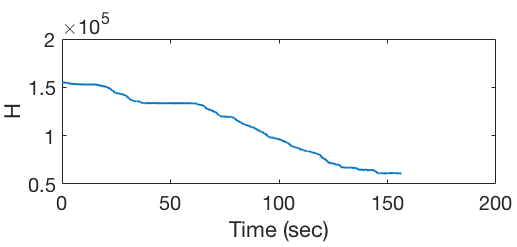
\includegraphics[width=0.4\textwidth]{entropy_experiment_aspect3by1.png}
	\caption{Experimental Environment Map Entropy}
	\label{fig:expH}
\end{figure}

The projected map used for both collision and exploration has several benefits. The robot measures walls and objects with the 3D map, and nicely represents these as occupied spaces with the 2D projected map. Additionally, the robot explores the space much faster than with two separate maps, primarily because the robot avoided repeatedly exploring spaces as with the entropy-only map in Section IV. This decision leads to a tradeoff; with the experiment shown here, the robot exploration did not consider low cells, particularly those near the ground. As a result, some floor regions are not captured by the 3D occupancy grid even though cells above the floor are well-known.
 
 The 3D mapping works very well in most scenarios, but exploration requires some tuning. Most importantly, the value of $d_\text{max}$ in \refeqn{bumpFun} has a major impact. A value of $5$m is selected to prioritize local exploration trajectories first. This value only increases if the maximum value of $d_\text{cell}$ exceeds $d_\text{max}$, in which $d_\text{max}$ is reassigned to $d_\text{cell}$.

% ATTENTION: left out patched segment size and polynomial order
\section{Conclusions and Future Work}

This paper covers the important aspects of exploring and mapping a 3D environment using exact inverse sensor models and expected entropies. The 3D mapping produces occupancy probabilities with depth sensor fusion from an arbitrary number sensors. Due to the computational difficulties of exploration in 3D, a 2D version of exploration is combined with 3D mapping. These are demonstrated with numerical simulations and experiments with an aerial vehicle.

There are two important future directions. One direction is a more complete 3D exploration considering the map expected information gain via measurement rays cast in 3D. This approach could better capture cells on the ground or vertically-nonuniform objects, but careful consideration must be placed on computational restrictions. Secondly, the 3D occupancy grid may be used by multiple robots for faster exploration.



%Our contribution will be
%        1.      proposing a method to combine 3D mapping and 2D exploration
%        2.      sensor fusion in mapping
%        3.      hardware/software for aerial exploration experiment.
%
%I suggest that the last few paragraphs are revised to emphasize the above. Perhaps, one paragraph for each of the above will be ideal. Also, we need to motivate why we are not doing full 3D exploration. Stress that we are proposing a computationally friendly approach to perform 3D mapping with projection using the fact there is less variation in the floor plan along the vertical direction.





% conference papers do not normally have an appendix


% use section* for acknowledgement
%\section*{Acknowledgment}
%
%
%The authors would like to thank...





% trigger a \newpage just before the given reference
% number - used to balance the columns on the last page
% adjust value as needed - may need to be readjusted if
% the document is modified later
%\IEEEtriggeratref{8}
% The "triggered" command can be changed if desired:
%\IEEEtriggercmd{\enlargethispage{-5in}}

% references section

% can use a bibliography generated by BibTeX as a .bbl file
% BibTeX documentation can be easily obtained at:
% http://www.ctan.org/tex-archive/biblio/bibtex/contrib/doc/
% The IEEEtran BibTeX style support page is at:
% http://www.michaelshell.org/tex/ieeetran/bibtex/
%\bibliography{BibSources}% accessible locally only
\bibliography{../../BibSources}% master source for all publications
\bibliographystyle{IEEEtran}
% argument is your BibTeX string definitions and bibliography database(s)
%\bibliography{IEEEabrv,../bib/paper}
%
% <OR> manually copy in the resultant .bbl file
% set second argument of \begin to the number of references
% (used to reserve space for the reference number labels box)
%\begin{thebibliography}{1}
%
%\bibitem{IEEEhowto:kopka}
%H.~Kopka and P.~W. Daly, \emph{A Guide to \LaTeX}, 3rd~ed.\hskip 1em plus
%  0.5em minus 0.4em\relax Harlow, England: Addison-Wesley, 1999.
%
%\end{thebibliography}




% that's all folks
\end{document}


